\batchmode
\documentclass[twoside]{book}

% Packages required by doxygen
\usepackage{fixltx2e}
\usepackage{calc}
\usepackage{doxygen}
\usepackage[export]{adjustbox} % also loads graphicx
\usepackage{graphicx}
\usepackage[utf8]{inputenc}
\usepackage{makeidx}
\usepackage{multicol}
\usepackage{multirow}
\PassOptionsToPackage{warn}{textcomp}
\usepackage{textcomp}
\usepackage[nointegrals]{wasysym}
\usepackage[table]{xcolor}

% Font selection
\usepackage[T1]{fontenc}
\usepackage[scaled=.90]{helvet}
\usepackage{courier}
\usepackage{amssymb}
\usepackage{sectsty}
\renewcommand{\familydefault}{\sfdefault}
\allsectionsfont{%
  \fontseries{bc}\selectfont%
  \color{darkgray}%
}
\renewcommand{\DoxyLabelFont}{%
  \fontseries{bc}\selectfont%
  \color{darkgray}%
}
\newcommand{\+}{\discretionary{\mbox{\scriptsize$\hookleftarrow$}}{}{}}

% Page & text layout
\usepackage{geometry}
\geometry{%
  a4paper,%
  top=2.5cm,%
  bottom=2.5cm,%
  left=2.5cm,%
  right=2.5cm%
}
\tolerance=750
\hfuzz=15pt
\hbadness=750
\setlength{\emergencystretch}{15pt}
\setlength{\parindent}{0cm}
\setlength{\parskip}{3ex plus 2ex minus 2ex}
\makeatletter
\renewcommand{\paragraph}{%
  \@startsection{paragraph}{4}{0ex}{-1.0ex}{1.0ex}{%
    \normalfont\normalsize\bfseries\SS@parafont%
  }%
}
\renewcommand{\subparagraph}{%
  \@startsection{subparagraph}{5}{0ex}{-1.0ex}{1.0ex}{%
    \normalfont\normalsize\bfseries\SS@subparafont%
  }%
}
\makeatother

% Headers & footers
\usepackage{fancyhdr}
\pagestyle{fancyplain}
\fancyhead[LE]{\fancyplain{}{\bfseries\thepage}}
\fancyhead[CE]{\fancyplain{}{}}
\fancyhead[RE]{\fancyplain{}{\bfseries\leftmark}}
\fancyhead[LO]{\fancyplain{}{\bfseries\rightmark}}
\fancyhead[CO]{\fancyplain{}{}}
\fancyhead[RO]{\fancyplain{}{\bfseries\thepage}}
\fancyfoot[LE]{\fancyplain{}{}}
\fancyfoot[CE]{\fancyplain{}{}}
\fancyfoot[RE]{\fancyplain{}{\bfseries\scriptsize Generated by Doxygen }}
\fancyfoot[LO]{\fancyplain{}{\bfseries\scriptsize Generated by Doxygen }}
\fancyfoot[CO]{\fancyplain{}{}}
\fancyfoot[RO]{\fancyplain{}{}}
\renewcommand{\footrulewidth}{0.4pt}
\renewcommand{\chaptermark}[1]{%
  \markboth{#1}{}%
}
\renewcommand{\sectionmark}[1]{%
  \markright{\thesection\ #1}%
}

% Indices & bibliography
\usepackage{natbib}
\usepackage[titles]{tocloft}
\setcounter{tocdepth}{3}
\setcounter{secnumdepth}{5}
\makeindex

% Hyperlinks (required, but should be loaded last)
\usepackage{ifpdf}
\ifpdf
  \usepackage[pdftex,pagebackref=true]{hyperref}
\else
  \usepackage[ps2pdf,pagebackref=true]{hyperref}
\fi
\hypersetup{%
  colorlinks=true,%
  linkcolor=blue,%
  citecolor=blue,%
  unicode%
}

% Custom commands
\newcommand{\clearemptydoublepage}{%
  \newpage{\pagestyle{empty}\cleardoublepage}%
}

\usepackage{caption}
\captionsetup{labelsep=space,justification=centering,font={bf},singlelinecheck=off,skip=4pt,position=top}

%===== C O N T E N T S =====

\begin{document}

% Titlepage & ToC
\hypersetup{pageanchor=false,
             bookmarksnumbered=true
            }
\pagenumbering{alph}
\pagenumbering{arabic}
\hypersetup{pageanchor=true}

%--- Begin generated contents ---
\chapter{A real fluid-\/structure interaction problem\+: Finite Reynolds number flow in an oscillating elastic ring.}
\label{index}\hypertarget{index}{}\hypertarget{index_q}{}\section{A few quick questions...}\label{index_q}
Since {\ttfamily oomph-\/lib} is developed as open-\/source software, any evidence that the code is being downloaded and used is very helpful for us as it helps to justify our continued work on this project.

We would therefore be extremely grateful if you could provide the information requested in the form below. Pressing the \char`\"{}submit\char`\"{} button will get you to the actual download page.

{\bfseries Note\+:} 
\begin{DoxyItemize}
\item All information will be treated as confidential. 
\item If you provide your email address and check the appropriate box we will add you to our mailing list to inform you of upgrades and bug fixes to the code. Rest assured that the mailing list is {\bfseries very low volume} -- we have better things to do than to bombard you with email. 
\item If you still feel reluctant to provide any of the information requested, feel free to enter some dummy input. The form will check that {\bfseries some} information has been entered but entering your name as \char`\"{}\+Joe Cool\char`\"{} is perfectly acceptable -- this is to discourage people from not providing the information simply because they are too lazy to type... 
\end{DoxyItemize}



 







 

 \hypertarget{index_pdf}{}\section{P\+D\+F file}\label{index_pdf}
A \href{../latex/refman.pdf}{\tt pdf version} of this document is available. \end{document}

\chapter{Namespace Index}
\section{Namespace List}
Here is a list of all namespaces with brief descriptions\+:\begin{DoxyCompactList}
\item\contentsline{section}{\hyperlink{namespaceGlobal__Physical__Variables}{Global\+\_\+\+Physical\+\_\+\+Variables} \\*Global variables that represent physical properties }{\pageref{namespaceGlobal__Physical__Variables}}{}
\item\contentsline{section}{\hyperlink{namespaceoomph}{oomph} }{\pageref{namespaceoomph}}{}
\item\contentsline{section}{\hyperlink{namespacePhysical__Variables}{Physical\+\_\+\+Variables} \\*Namespace for the solution of 2D linear shell equation }{\pageref{namespacePhysical__Variables}}{}
\end{DoxyCompactList}

\chapter{Hierarchical Index}
\section{Class Hierarchy}
This inheritance list is sorted roughly, but not completely, alphabetically\+:\begin{DoxyCompactList}
\item Problem\begin{DoxyCompactList}
\item \contentsline{section}{Unstructured\+Solid\+Problem$<$ E\+L\+E\+M\+E\+NT $>$}{\pageref{classUnstructuredSolidProblem}}{}
\end{DoxyCompactList}
\end{DoxyCompactList}

\chapter{Class Index}
\section{Class List}
Here are the classes, structs, unions and interfaces with brief descriptions\+:\begin{DoxyCompactList}
\item\contentsline{section}{\hyperlink{classPMLProblem}{P\+M\+L\+Problem$<$ E\+L\+E\+M\+E\+N\+T $>$} }{\pageref{classPMLProblem}}{}
\item\contentsline{section}{\hyperlink{classGlobalParameters_1_1TestPMLMapping}{Global\+Parameters\+::\+Test\+P\+M\+L\+Mapping} }{\pageref{classGlobalParameters_1_1TestPMLMapping}}{}
\end{DoxyCompactList}

\chapter{File Index}
\section{File List}
Here is a list of all files with brief descriptions\+:\begin{DoxyCompactList}
\item\contentsline{section}{\hyperlink{jeffery__orbit_8cc}{jeffery\+\_\+orbit.\+cc} }{\pageref{jeffery__orbit_8cc}}{}
\item\contentsline{section}{\hyperlink{jeffery__orbit_8txt__doxygenified_8h}{jeffery\+\_\+orbit.\+txt\+\_\+doxygenified.\+h} }{\pageref{jeffery__orbit_8txt__doxygenified_8h}}{}
\item\contentsline{section}{\hyperlink{my__taylor__hood__elements_8h}{my\+\_\+taylor\+\_\+hood\+\_\+elements.\+h} }{\pageref{my__taylor__hood__elements_8h}}{}
\end{DoxyCompactList}

\chapter{Namespace Documentation}
\hypertarget{namespaceGlobal__Physical__Variables}{}\section{Global\+\_\+\+Physical\+\_\+\+Variables Namespace Reference}
\label{namespaceGlobal__Physical__Variables}\index{Global\+\_\+\+Physical\+\_\+\+Variables@{Global\+\_\+\+Physical\+\_\+\+Variables}}


Namespace for physical parameters.  


\subsection*{Functions}
\begin{DoxyCompactItemize}
\item 
Vector$<$ double $>$ \hyperlink{namespaceGlobal__Physical__Variables_afae321364975eb56688ad13abc8ed6b7}{Gravity} (2)
\begin{DoxyCompactList}\small\item\em Gravity vector. \end{DoxyCompactList}\item 
void \hyperlink{namespaceGlobal__Physical__Variables_a87da705b8a46bed337cf5dbdd788b87b}{body\+\_\+force} (const double \&time, const Vector$<$ double $>$ \&x, Vector$<$ double $>$ \&result)
\begin{DoxyCompactList}\small\item\em Functional body force. \end{DoxyCompactList}\item 
void \hyperlink{namespaceGlobal__Physical__Variables_a9780d615ae07c4e00a436ab2973b54e6}{zero\+\_\+body\+\_\+force} (const double \&time, const Vector$<$ double $>$ \&x, Vector$<$ double $>$ \&result)
\begin{DoxyCompactList}\small\item\em Zero functional body force. \end{DoxyCompactList}\end{DoxyCompactItemize}
\subsection*{Variables}
\begin{DoxyCompactItemize}
\item 
double \hyperlink{namespaceGlobal__Physical__Variables_ab814e627d2eb5bc50318879d19ab16b9}{Re} =100
\begin{DoxyCompactList}\small\item\em Reynolds number. \end{DoxyCompactList}\item 
double \hyperlink{namespaceGlobal__Physical__Variables_ab1a845a672b4d74b304639a976dc65c6}{Re\+\_\+inv\+Fr} =100
\begin{DoxyCompactList}\small\item\em Reynolds/\+Froude number. \end{DoxyCompactList}\end{DoxyCompactItemize}


\subsection{Detailed Description}
Namespace for physical parameters. 

\subsection{Function Documentation}
\mbox{\Hypertarget{namespaceGlobal__Physical__Variables_a87da705b8a46bed337cf5dbdd788b87b}\label{namespaceGlobal__Physical__Variables_a87da705b8a46bed337cf5dbdd788b87b}} 
\index{Global\+\_\+\+Physical\+\_\+\+Variables@{Global\+\_\+\+Physical\+\_\+\+Variables}!body\+\_\+force@{body\+\_\+force}}
\index{body\+\_\+force@{body\+\_\+force}!Global\+\_\+\+Physical\+\_\+\+Variables@{Global\+\_\+\+Physical\+\_\+\+Variables}}
\subsubsection{\texorpdfstring{body\+\_\+force()}{body\_force()}}
{\footnotesize\ttfamily void Global\+\_\+\+Physical\+\_\+\+Variables\+::body\+\_\+force (\begin{DoxyParamCaption}\item[{const double \&}]{time,  }\item[{const Vector$<$ double $>$ \&}]{x,  }\item[{Vector$<$ double $>$ \&}]{result }\end{DoxyParamCaption})}



Functional body force. 



Definition at line 62 of file circular\+\_\+driven\+\_\+cavity.\+cc.



References Re\+\_\+inv\+Fr.



Referenced by main().

\mbox{\Hypertarget{namespaceGlobal__Physical__Variables_afae321364975eb56688ad13abc8ed6b7}\label{namespaceGlobal__Physical__Variables_afae321364975eb56688ad13abc8ed6b7}} 
\index{Global\+\_\+\+Physical\+\_\+\+Variables@{Global\+\_\+\+Physical\+\_\+\+Variables}!Gravity@{Gravity}}
\index{Gravity@{Gravity}!Global\+\_\+\+Physical\+\_\+\+Variables@{Global\+\_\+\+Physical\+\_\+\+Variables}}
\subsubsection{\texorpdfstring{Gravity()}{Gravity()}}
{\footnotesize\ttfamily Vector$<$double$>$ Global\+\_\+\+Physical\+\_\+\+Variables\+::\+Gravity (\begin{DoxyParamCaption}\item[{2}]{ }\end{DoxyParamCaption})}



Gravity vector. 



Referenced by main(), and Quarter\+Circle\+Driven\+Cavity\+Problem$<$ E\+L\+E\+M\+E\+N\+T $>$\+::\+Quarter\+Circle\+Driven\+Cavity\+Problem().

\mbox{\Hypertarget{namespaceGlobal__Physical__Variables_a9780d615ae07c4e00a436ab2973b54e6}\label{namespaceGlobal__Physical__Variables_a9780d615ae07c4e00a436ab2973b54e6}} 
\index{Global\+\_\+\+Physical\+\_\+\+Variables@{Global\+\_\+\+Physical\+\_\+\+Variables}!zero\+\_\+body\+\_\+force@{zero\+\_\+body\+\_\+force}}
\index{zero\+\_\+body\+\_\+force@{zero\+\_\+body\+\_\+force}!Global\+\_\+\+Physical\+\_\+\+Variables@{Global\+\_\+\+Physical\+\_\+\+Variables}}
\subsubsection{\texorpdfstring{zero\+\_\+body\+\_\+force()}{zero\_body\_force()}}
{\footnotesize\ttfamily void Global\+\_\+\+Physical\+\_\+\+Variables\+::zero\+\_\+body\+\_\+force (\begin{DoxyParamCaption}\item[{const double \&}]{time,  }\item[{const Vector$<$ double $>$ \&}]{x,  }\item[{Vector$<$ double $>$ \&}]{result }\end{DoxyParamCaption})}



Zero functional body force. 



Definition at line 70 of file circular\+\_\+driven\+\_\+cavity.\+cc.



Referenced by main().



\subsection{Variable Documentation}
\mbox{\Hypertarget{namespaceGlobal__Physical__Variables_ab814e627d2eb5bc50318879d19ab16b9}\label{namespaceGlobal__Physical__Variables_ab814e627d2eb5bc50318879d19ab16b9}} 
\index{Global\+\_\+\+Physical\+\_\+\+Variables@{Global\+\_\+\+Physical\+\_\+\+Variables}!Re@{Re}}
\index{Re@{Re}!Global\+\_\+\+Physical\+\_\+\+Variables@{Global\+\_\+\+Physical\+\_\+\+Variables}}
\subsubsection{\texorpdfstring{Re}{Re}}
{\footnotesize\ttfamily double Global\+\_\+\+Physical\+\_\+\+Variables\+::\+Re =100}



Reynolds number. 



Definition at line 53 of file circular\+\_\+driven\+\_\+cavity.\+cc.



Referenced by Quarter\+Circle\+Driven\+Cavity\+Problem$<$ E\+L\+E\+M\+E\+N\+T $>$\+::\+Quarter\+Circle\+Driven\+Cavity\+Problem().

\mbox{\Hypertarget{namespaceGlobal__Physical__Variables_ab1a845a672b4d74b304639a976dc65c6}\label{namespaceGlobal__Physical__Variables_ab1a845a672b4d74b304639a976dc65c6}} 
\index{Global\+\_\+\+Physical\+\_\+\+Variables@{Global\+\_\+\+Physical\+\_\+\+Variables}!Re\+\_\+inv\+Fr@{Re\+\_\+inv\+Fr}}
\index{Re\+\_\+inv\+Fr@{Re\+\_\+inv\+Fr}!Global\+\_\+\+Physical\+\_\+\+Variables@{Global\+\_\+\+Physical\+\_\+\+Variables}}
\subsubsection{\texorpdfstring{Re\+\_\+inv\+Fr}{Re\_invFr}}
{\footnotesize\ttfamily double Global\+\_\+\+Physical\+\_\+\+Variables\+::\+Re\+\_\+inv\+Fr =100}



Reynolds/\+Froude number. 



Definition at line 56 of file circular\+\_\+driven\+\_\+cavity.\+cc.



Referenced by body\+\_\+force(), and Quarter\+Circle\+Driven\+Cavity\+Problem$<$ E\+L\+E\+M\+E\+N\+T $>$\+::\+Quarter\+Circle\+Driven\+Cavity\+Problem().


\hypertarget{namespaceoomph}{}\section{oomph Namespace Reference}
\label{namespaceoomph}\index{oomph@{oomph}}
\subsection*{Classes}
\begin{DoxyCompactItemize}
\item 
class \hyperlink{classoomph_1_1BellShellElement}{Bell\+Shell\+Element}
\begin{DoxyCompactList}\small\item\em \hyperlink{classoomph_1_1BellShellElement}{Bell\+Shell\+Element} elements are with subparametric interpolation for the function. \end{DoxyCompactList}\item 
class \hyperlink{classoomph_1_1FaceGeometry_3_01BellShellElement_3_01DIM_00_01NNODE__1D_01_4_01_4}{Face\+Geometry$<$ Bell\+Shell\+Element$<$ D\+I\+M, N\+N\+O\+D\+E\+\_\+1\+D $>$ $>$}
\item 
class \hyperlink{classoomph_1_1MyShellEquations}{My\+Shell\+Equations}
\item 
class \hyperlink{classoomph_1_1Plate}{Plate}
\begin{DoxyCompactList}\small\item\em Elliptical tube with half axes a and b. \end{DoxyCompactList}\end{DoxyCompactItemize}

\hypertarget{namespaceoomph_1_1SarahBL}{}\section{oomph\+:\+:Sarah\+BL Namespace Reference}
\label{namespaceoomph_1_1SarahBL}\index{oomph\+::\+Sarah\+BL@{oomph\+::\+Sarah\+BL}}


Sarah\textquotesingle{}s boundary layer solution for flow in oscillating ring.  


\subsection*{Functions}
\begin{DoxyCompactItemize}
\item 
double \hyperlink{namespaceoomph_1_1SarahBL_a38ddc42a9eb5dee8b355795e28df0e45}{Diss\+\_\+sarah} (double rho, double zeta, double t)
\item 
double \hyperlink{namespaceoomph_1_1SarahBL_a3cb8715d5fa21d7dbff8151e90df4200}{Kin\+\_\+energy\+\_\+sarah} (double t)
\item 
double \hyperlink{namespaceoomph_1_1SarahBL_a8c9f906a629a8eae5eca6346ccf07040}{P\+\_\+sarah} (double rho, double zeta, double t)
\item 
double \hyperlink{namespaceoomph_1_1SarahBL_a8dccddb7ea423d14b6fa8dc9bdb9eca7}{Total\+\_\+\+Diss\+\_\+lead\+\_\+sarah} (double t)
\item 
double \hyperlink{namespaceoomph_1_1SarahBL_abcbefc8bfea90a749dcb6961d9d5c0a0}{Total\+\_\+\+Diss\+\_\+sarah} (double t)
\item 
double \hyperlink{namespaceoomph_1_1SarahBL_a702395898e24e2ff65f724a79b88f63b}{U\+\_\+sarah} (double rho, double zeta, double t)
\item 
double \hyperlink{namespaceoomph_1_1SarahBL_afe2672fb083e5cd566f80d7a0f20df94}{V\+\_\+sarah} (double rho, double zeta, double t)
\item 
double \hyperlink{namespaceoomph_1_1SarahBL_a18945b08e90840028742a9ca2aed94c9}{X\+\_\+sarah} (double rho, double zeta, double t)
\item 
double \hyperlink{namespaceoomph_1_1SarahBL_a95d6eff2fce4d76da4adda6acaea78be}{Y\+\_\+sarah} (double rho, double zeta, double t)
\item 
void \hyperlink{namespaceoomph_1_1SarahBL_a8dadcc240f5e25e9ba10936749678ff6}{buckled\+\_\+ring\+\_\+residual} (const Vector$<$ double $>$ \&params, const Vector$<$ double $>$ \&unknowns, Vector$<$ double $>$ \&residuals)
\begin{DoxyCompactList}\small\item\em Residual function for buckled ring. \end{DoxyCompactList}\item 
void \hyperlink{namespaceoomph_1_1SarahBL_aa198aa1de07bb9a2eac422ed63010bc4}{exact\+\_\+soln} (const double \&time, const Vector$<$ double $>$ \&x, Vector$<$ double $>$ \&soln)
\begin{DoxyCompactList}\small\item\em Exact solution\+: x,y,u,v,p. \end{DoxyCompactList}\item 
void \hyperlink{namespaceoomph_1_1SarahBL_a80c7c03073f6436ace00d2b2c5bfa501}{full\+\_\+exact\+\_\+soln} (const double \&time, const Vector$<$ double $>$ \&x, Vector$<$ double $>$ \&soln)
\begin{DoxyCompactList}\small\item\em Full exact solution\+: x,y,u,v,p,du/dt,dv/dt,diss. \end{DoxyCompactList}\end{DoxyCompactItemize}
\subsection*{Variables}
\begin{DoxyCompactItemize}
\item 
double \hyperlink{namespaceoomph_1_1SarahBL_a21bfe7e71f0baa62022d1ecc9bd175de}{epsilon}
\item 
double \hyperlink{namespaceoomph_1_1SarahBL_ab07de8eb877306afdc10ba4a17c6406b}{alpha}
\item 
double \hyperlink{namespaceoomph_1_1SarahBL_a5b48abf91ca062e8bfeab87f1d4a9499}{A}
\item 
double \hyperlink{namespaceoomph_1_1SarahBL_a370241de5869d0f53fc7cd17858bfbfe}{Omega}
\item 
double \hyperlink{namespaceoomph_1_1SarahBL_a3f2e6fdba588e1883d317f6e0cd7f32f}{N}
\end{DoxyCompactItemize}


\subsection{Detailed Description}
Sarah\textquotesingle{}s boundary layer solution for flow in oscillating ring. 

\subsection{Function Documentation}
\mbox{\Hypertarget{namespaceoomph_1_1SarahBL_a8dadcc240f5e25e9ba10936749678ff6}\label{namespaceoomph_1_1SarahBL_a8dadcc240f5e25e9ba10936749678ff6}} 
\index{oomph\+::\+Sarah\+BL@{oomph\+::\+Sarah\+BL}!buckled\+\_\+ring\+\_\+residual@{buckled\+\_\+ring\+\_\+residual}}
\index{buckled\+\_\+ring\+\_\+residual@{buckled\+\_\+ring\+\_\+residual}!oomph\+::\+Sarah\+BL@{oomph\+::\+Sarah\+BL}}
\subsubsection{\texorpdfstring{buckled\+\_\+ring\+\_\+residual()}{buckled\_ring\_residual()}}
{\footnotesize\ttfamily void oomph\+::\+Sarah\+B\+L\+::buckled\+\_\+ring\+\_\+residual (\begin{DoxyParamCaption}\item[{const Vector$<$ double $>$ \&}]{params,  }\item[{const Vector$<$ double $>$ \&}]{unknowns,  }\item[{Vector$<$ double $>$ \&}]{residuals }\end{DoxyParamCaption})}



Residual function for buckled ring. 



Definition at line 399 of file osc\+\_\+ring\+\_\+sarah\+\_\+asymptotics.\+h.



References X\+\_\+sarah(), and Y\+\_\+sarah().



Referenced by exact\+\_\+soln(), and full\+\_\+exact\+\_\+soln().

\mbox{\Hypertarget{namespaceoomph_1_1SarahBL_a38ddc42a9eb5dee8b355795e28df0e45}\label{namespaceoomph_1_1SarahBL_a38ddc42a9eb5dee8b355795e28df0e45}} 
\index{oomph\+::\+Sarah\+BL@{oomph\+::\+Sarah\+BL}!Diss\+\_\+sarah@{Diss\+\_\+sarah}}
\index{Diss\+\_\+sarah@{Diss\+\_\+sarah}!oomph\+::\+Sarah\+BL@{oomph\+::\+Sarah\+BL}}
\subsubsection{\texorpdfstring{Diss\+\_\+sarah()}{Diss\_sarah()}}
{\footnotesize\ttfamily double oomph\+::\+Sarah\+B\+L\+::\+Diss\+\_\+sarah (\begin{DoxyParamCaption}\item[{double}]{rho,  }\item[{double}]{zeta,  }\item[{double}]{t }\end{DoxyParamCaption})}



Definition at line 51 of file osc\+\_\+ring\+\_\+sarah\+\_\+asymptotics.\+h.



References A, alpha, epsilon, and Omega.



Referenced by full\+\_\+exact\+\_\+soln().

\mbox{\Hypertarget{namespaceoomph_1_1SarahBL_aa198aa1de07bb9a2eac422ed63010bc4}\label{namespaceoomph_1_1SarahBL_aa198aa1de07bb9a2eac422ed63010bc4}} 
\index{oomph\+::\+Sarah\+BL@{oomph\+::\+Sarah\+BL}!exact\+\_\+soln@{exact\+\_\+soln}}
\index{exact\+\_\+soln@{exact\+\_\+soln}!oomph\+::\+Sarah\+BL@{oomph\+::\+Sarah\+BL}}
\subsubsection{\texorpdfstring{exact\+\_\+soln()}{exact\_soln()}}
{\footnotesize\ttfamily void oomph\+::\+Sarah\+B\+L\+::exact\+\_\+soln (\begin{DoxyParamCaption}\item[{const double \&}]{time,  }\item[{const Vector$<$ double $>$ \&}]{x,  }\item[{Vector$<$ double $>$ \&}]{soln }\end{DoxyParamCaption})}



Exact solution\+: x,y,u,v,p. 



Definition at line 422 of file osc\+\_\+ring\+\_\+sarah\+\_\+asymptotics.\+h.



References alpha, buckled\+\_\+ring\+\_\+residual(), P\+\_\+sarah(), U\+\_\+sarah(), V\+\_\+sarah(), X\+\_\+sarah(), and Y\+\_\+sarah().



Referenced by Osc\+Ring\+N\+St\+Problem$<$ E\+L\+E\+M\+E\+N\+T $>$\+::doc\+\_\+solution().

\mbox{\Hypertarget{namespaceoomph_1_1SarahBL_a80c7c03073f6436ace00d2b2c5bfa501}\label{namespaceoomph_1_1SarahBL_a80c7c03073f6436ace00d2b2c5bfa501}} 
\index{oomph\+::\+Sarah\+BL@{oomph\+::\+Sarah\+BL}!full\+\_\+exact\+\_\+soln@{full\+\_\+exact\+\_\+soln}}
\index{full\+\_\+exact\+\_\+soln@{full\+\_\+exact\+\_\+soln}!oomph\+::\+Sarah\+BL@{oomph\+::\+Sarah\+BL}}
\subsubsection{\texorpdfstring{full\+\_\+exact\+\_\+soln()}{full\_exact\_soln()}}
{\footnotesize\ttfamily void oomph\+::\+Sarah\+B\+L\+::full\+\_\+exact\+\_\+soln (\begin{DoxyParamCaption}\item[{const double \&}]{time,  }\item[{const Vector$<$ double $>$ \&}]{x,  }\item[{Vector$<$ double $>$ \&}]{soln }\end{DoxyParamCaption})}



Full exact solution\+: x,y,u,v,p,du/dt,dv/dt,diss. 



Definition at line 484 of file osc\+\_\+ring\+\_\+sarah\+\_\+asymptotics.\+h.



References alpha, buckled\+\_\+ring\+\_\+residual(), Diss\+\_\+sarah(), P\+\_\+sarah(), U\+\_\+sarah(), V\+\_\+sarah(), X\+\_\+sarah(), and Y\+\_\+sarah().



Referenced by Osc\+Ring\+N\+St\+Problem$<$ E\+L\+E\+M\+E\+N\+T $>$\+::doc\+\_\+solution(), and main().

\mbox{\Hypertarget{namespaceoomph_1_1SarahBL_a3cb8715d5fa21d7dbff8151e90df4200}\label{namespaceoomph_1_1SarahBL_a3cb8715d5fa21d7dbff8151e90df4200}} 
\index{oomph\+::\+Sarah\+BL@{oomph\+::\+Sarah\+BL}!Kin\+\_\+energy\+\_\+sarah@{Kin\+\_\+energy\+\_\+sarah}}
\index{Kin\+\_\+energy\+\_\+sarah@{Kin\+\_\+energy\+\_\+sarah}!oomph\+::\+Sarah\+BL@{oomph\+::\+Sarah\+BL}}
\subsubsection{\texorpdfstring{Kin\+\_\+energy\+\_\+sarah()}{Kin\_energy\_sarah()}}
{\footnotesize\ttfamily double oomph\+::\+Sarah\+B\+L\+::\+Kin\+\_\+energy\+\_\+sarah (\begin{DoxyParamCaption}\item[{double}]{t }\end{DoxyParamCaption})}



Definition at line 94 of file osc\+\_\+ring\+\_\+sarah\+\_\+asymptotics.\+h.



References A, alpha, epsilon, and Omega.



Referenced by Osc\+Ring\+N\+St\+Problem$<$ E\+L\+E\+M\+E\+N\+T $>$\+::doc\+\_\+solution().

\mbox{\Hypertarget{namespaceoomph_1_1SarahBL_a8c9f906a629a8eae5eca6346ccf07040}\label{namespaceoomph_1_1SarahBL_a8c9f906a629a8eae5eca6346ccf07040}} 
\index{oomph\+::\+Sarah\+BL@{oomph\+::\+Sarah\+BL}!P\+\_\+sarah@{P\+\_\+sarah}}
\index{P\+\_\+sarah@{P\+\_\+sarah}!oomph\+::\+Sarah\+BL@{oomph\+::\+Sarah\+BL}}
\subsubsection{\texorpdfstring{P\+\_\+sarah()}{P\_sarah()}}
{\footnotesize\ttfamily double oomph\+::\+Sarah\+B\+L\+::\+P\+\_\+sarah (\begin{DoxyParamCaption}\item[{double}]{rho,  }\item[{double}]{zeta,  }\item[{double}]{t }\end{DoxyParamCaption})}



Definition at line 134 of file osc\+\_\+ring\+\_\+sarah\+\_\+asymptotics.\+h.



References Omega.



Referenced by exact\+\_\+soln(), and full\+\_\+exact\+\_\+soln().

\mbox{\Hypertarget{namespaceoomph_1_1SarahBL_a8dccddb7ea423d14b6fa8dc9bdb9eca7}\label{namespaceoomph_1_1SarahBL_a8dccddb7ea423d14b6fa8dc9bdb9eca7}} 
\index{oomph\+::\+Sarah\+BL@{oomph\+::\+Sarah\+BL}!Total\+\_\+\+Diss\+\_\+lead\+\_\+sarah@{Total\+\_\+\+Diss\+\_\+lead\+\_\+sarah}}
\index{Total\+\_\+\+Diss\+\_\+lead\+\_\+sarah@{Total\+\_\+\+Diss\+\_\+lead\+\_\+sarah}!oomph\+::\+Sarah\+BL@{oomph\+::\+Sarah\+BL}}
\subsubsection{\texorpdfstring{Total\+\_\+\+Diss\+\_\+lead\+\_\+sarah()}{Total\_Diss\_lead\_sarah()}}
{\footnotesize\ttfamily double oomph\+::\+Sarah\+B\+L\+::\+Total\+\_\+\+Diss\+\_\+lead\+\_\+sarah (\begin{DoxyParamCaption}\item[{double}]{t }\end{DoxyParamCaption})}



Definition at line 157 of file osc\+\_\+ring\+\_\+sarah\+\_\+asymptotics.\+h.



References epsilon, and Omega.

\mbox{\Hypertarget{namespaceoomph_1_1SarahBL_abcbefc8bfea90a749dcb6961d9d5c0a0}\label{namespaceoomph_1_1SarahBL_abcbefc8bfea90a749dcb6961d9d5c0a0}} 
\index{oomph\+::\+Sarah\+BL@{oomph\+::\+Sarah\+BL}!Total\+\_\+\+Diss\+\_\+sarah@{Total\+\_\+\+Diss\+\_\+sarah}}
\index{Total\+\_\+\+Diss\+\_\+sarah@{Total\+\_\+\+Diss\+\_\+sarah}!oomph\+::\+Sarah\+BL@{oomph\+::\+Sarah\+BL}}
\subsubsection{\texorpdfstring{Total\+\_\+\+Diss\+\_\+sarah()}{Total\_Diss\_sarah()}}
{\footnotesize\ttfamily double oomph\+::\+Sarah\+B\+L\+::\+Total\+\_\+\+Diss\+\_\+sarah (\begin{DoxyParamCaption}\item[{double}]{t }\end{DoxyParamCaption})}



Definition at line 185 of file osc\+\_\+ring\+\_\+sarah\+\_\+asymptotics.\+h.



References A, epsilon, and Omega.



Referenced by Osc\+Ring\+N\+St\+Problem$<$ E\+L\+E\+M\+E\+N\+T $>$\+::doc\+\_\+solution().

\mbox{\Hypertarget{namespaceoomph_1_1SarahBL_a702395898e24e2ff65f724a79b88f63b}\label{namespaceoomph_1_1SarahBL_a702395898e24e2ff65f724a79b88f63b}} 
\index{oomph\+::\+Sarah\+BL@{oomph\+::\+Sarah\+BL}!U\+\_\+sarah@{U\+\_\+sarah}}
\index{U\+\_\+sarah@{U\+\_\+sarah}!oomph\+::\+Sarah\+BL@{oomph\+::\+Sarah\+BL}}
\subsubsection{\texorpdfstring{U\+\_\+sarah()}{U\_sarah()}}
{\footnotesize\ttfamily double oomph\+::\+Sarah\+B\+L\+::\+U\+\_\+sarah (\begin{DoxyParamCaption}\item[{double}]{rho,  }\item[{double}]{zeta,  }\item[{double}]{t }\end{DoxyParamCaption})}



Definition at line 218 of file osc\+\_\+ring\+\_\+sarah\+\_\+asymptotics.\+h.



References A, alpha, and epsilon.



Referenced by exact\+\_\+soln(), and full\+\_\+exact\+\_\+soln().

\mbox{\Hypertarget{namespaceoomph_1_1SarahBL_afe2672fb083e5cd566f80d7a0f20df94}\label{namespaceoomph_1_1SarahBL_afe2672fb083e5cd566f80d7a0f20df94}} 
\index{oomph\+::\+Sarah\+BL@{oomph\+::\+Sarah\+BL}!V\+\_\+sarah@{V\+\_\+sarah}}
\index{V\+\_\+sarah@{V\+\_\+sarah}!oomph\+::\+Sarah\+BL@{oomph\+::\+Sarah\+BL}}
\subsubsection{\texorpdfstring{V\+\_\+sarah()}{V\_sarah()}}
{\footnotesize\ttfamily double oomph\+::\+Sarah\+B\+L\+::\+V\+\_\+sarah (\begin{DoxyParamCaption}\item[{double}]{rho,  }\item[{double}]{zeta,  }\item[{double}]{t }\end{DoxyParamCaption})}



Definition at line 287 of file osc\+\_\+ring\+\_\+sarah\+\_\+asymptotics.\+h.



References A, alpha, and epsilon.



Referenced by exact\+\_\+soln(), and full\+\_\+exact\+\_\+soln().

\mbox{\Hypertarget{namespaceoomph_1_1SarahBL_a18945b08e90840028742a9ca2aed94c9}\label{namespaceoomph_1_1SarahBL_a18945b08e90840028742a9ca2aed94c9}} 
\index{oomph\+::\+Sarah\+BL@{oomph\+::\+Sarah\+BL}!X\+\_\+sarah@{X\+\_\+sarah}}
\index{X\+\_\+sarah@{X\+\_\+sarah}!oomph\+::\+Sarah\+BL@{oomph\+::\+Sarah\+BL}}
\subsubsection{\texorpdfstring{X\+\_\+sarah()}{X\_sarah()}}
{\footnotesize\ttfamily double oomph\+::\+Sarah\+B\+L\+::\+X\+\_\+sarah (\begin{DoxyParamCaption}\item[{double}]{rho,  }\item[{double}]{zeta,  }\item[{double}]{t }\end{DoxyParamCaption})}



Definition at line 356 of file osc\+\_\+ring\+\_\+sarah\+\_\+asymptotics.\+h.



Referenced by buckled\+\_\+ring\+\_\+residual(), exact\+\_\+soln(), and full\+\_\+exact\+\_\+soln().

\mbox{\Hypertarget{namespaceoomph_1_1SarahBL_a95d6eff2fce4d76da4adda6acaea78be}\label{namespaceoomph_1_1SarahBL_a95d6eff2fce4d76da4adda6acaea78be}} 
\index{oomph\+::\+Sarah\+BL@{oomph\+::\+Sarah\+BL}!Y\+\_\+sarah@{Y\+\_\+sarah}}
\index{Y\+\_\+sarah@{Y\+\_\+sarah}!oomph\+::\+Sarah\+BL@{oomph\+::\+Sarah\+BL}}
\subsubsection{\texorpdfstring{Y\+\_\+sarah()}{Y\_sarah()}}
{\footnotesize\ttfamily double oomph\+::\+Sarah\+B\+L\+::\+Y\+\_\+sarah (\begin{DoxyParamCaption}\item[{double}]{rho,  }\item[{double}]{zeta,  }\item[{double}]{t }\end{DoxyParamCaption})}



Definition at line 377 of file osc\+\_\+ring\+\_\+sarah\+\_\+asymptotics.\+h.



Referenced by buckled\+\_\+ring\+\_\+residual(), exact\+\_\+soln(), and full\+\_\+exact\+\_\+soln().



\subsection{Variable Documentation}
\mbox{\Hypertarget{namespaceoomph_1_1SarahBL_a5b48abf91ca062e8bfeab87f1d4a9499}\label{namespaceoomph_1_1SarahBL_a5b48abf91ca062e8bfeab87f1d4a9499}} 
\index{oomph\+::\+Sarah\+BL@{oomph\+::\+Sarah\+BL}!A@{A}}
\index{A@{A}!oomph\+::\+Sarah\+BL@{oomph\+::\+Sarah\+BL}}
\subsubsection{\texorpdfstring{A}{A}}
{\footnotesize\ttfamily double oomph\+::\+Sarah\+B\+L\+::A}



Definition at line 47 of file osc\+\_\+ring\+\_\+sarah\+\_\+asymptotics.\+h.



Referenced by Diss\+\_\+sarah(), Kin\+\_\+energy\+\_\+sarah(), Osc\+Ring\+N\+St\+Problem$<$ E\+L\+E\+M\+E\+N\+T $>$\+::\+Osc\+Ring\+N\+St\+Problem(), Total\+\_\+\+Diss\+\_\+sarah(), U\+\_\+sarah(), and V\+\_\+sarah().

\mbox{\Hypertarget{namespaceoomph_1_1SarahBL_ab07de8eb877306afdc10ba4a17c6406b}\label{namespaceoomph_1_1SarahBL_ab07de8eb877306afdc10ba4a17c6406b}} 
\index{oomph\+::\+Sarah\+BL@{oomph\+::\+Sarah\+BL}!alpha@{alpha}}
\index{alpha@{alpha}!oomph\+::\+Sarah\+BL@{oomph\+::\+Sarah\+BL}}
\subsubsection{\texorpdfstring{alpha}{alpha}}
{\footnotesize\ttfamily double oomph\+::\+Sarah\+B\+L\+::alpha}



Definition at line 47 of file osc\+\_\+ring\+\_\+sarah\+\_\+asymptotics.\+h.



Referenced by Diss\+\_\+sarah(), exact\+\_\+soln(), full\+\_\+exact\+\_\+soln(), Kin\+\_\+energy\+\_\+sarah(), Osc\+Ring\+N\+St\+Problem$<$ E\+L\+E\+M\+E\+N\+T $>$\+::\+Osc\+Ring\+N\+St\+Problem(), U\+\_\+sarah(), and V\+\_\+sarah().

\mbox{\Hypertarget{namespaceoomph_1_1SarahBL_a21bfe7e71f0baa62022d1ecc9bd175de}\label{namespaceoomph_1_1SarahBL_a21bfe7e71f0baa62022d1ecc9bd175de}} 
\index{oomph\+::\+Sarah\+BL@{oomph\+::\+Sarah\+BL}!epsilon@{epsilon}}
\index{epsilon@{epsilon}!oomph\+::\+Sarah\+BL@{oomph\+::\+Sarah\+BL}}
\subsubsection{\texorpdfstring{epsilon}{epsilon}}
{\footnotesize\ttfamily double oomph\+::\+Sarah\+B\+L\+::epsilon}



Definition at line 47 of file osc\+\_\+ring\+\_\+sarah\+\_\+asymptotics.\+h.



Referenced by Diss\+\_\+sarah(), Kin\+\_\+energy\+\_\+sarah(), Osc\+Ring\+N\+St\+Problem$<$ E\+L\+E\+M\+E\+N\+T $>$\+::\+Osc\+Ring\+N\+St\+Problem(), Total\+\_\+\+Diss\+\_\+lead\+\_\+sarah(), Total\+\_\+\+Diss\+\_\+sarah(), U\+\_\+sarah(), and V\+\_\+sarah().

\mbox{\Hypertarget{namespaceoomph_1_1SarahBL_a3f2e6fdba588e1883d317f6e0cd7f32f}\label{namespaceoomph_1_1SarahBL_a3f2e6fdba588e1883d317f6e0cd7f32f}} 
\index{oomph\+::\+Sarah\+BL@{oomph\+::\+Sarah\+BL}!N@{N}}
\index{N@{N}!oomph\+::\+Sarah\+BL@{oomph\+::\+Sarah\+BL}}
\subsubsection{\texorpdfstring{N}{N}}
{\footnotesize\ttfamily double oomph\+::\+Sarah\+B\+L\+::N}



Definition at line 47 of file osc\+\_\+ring\+\_\+sarah\+\_\+asymptotics.\+h.



Referenced by F\+S\+I\+Ring\+Problem\+::\+F\+S\+I\+Ring\+Problem(), and Osc\+Ring\+N\+St\+Problem$<$ E\+L\+E\+M\+E\+N\+T $>$\+::\+Osc\+Ring\+N\+St\+Problem().

\mbox{\Hypertarget{namespaceoomph_1_1SarahBL_a370241de5869d0f53fc7cd17858bfbfe}\label{namespaceoomph_1_1SarahBL_a370241de5869d0f53fc7cd17858bfbfe}} 
\index{oomph\+::\+Sarah\+BL@{oomph\+::\+Sarah\+BL}!Omega@{Omega}}
\index{Omega@{Omega}!oomph\+::\+Sarah\+BL@{oomph\+::\+Sarah\+BL}}
\subsubsection{\texorpdfstring{Omega}{Omega}}
{\footnotesize\ttfamily double oomph\+::\+Sarah\+B\+L\+::\+Omega}



Definition at line 47 of file osc\+\_\+ring\+\_\+sarah\+\_\+asymptotics.\+h.



Referenced by Diss\+\_\+sarah(), Kin\+\_\+energy\+\_\+sarah(), Osc\+Ring\+N\+St\+Problem$<$ E\+L\+E\+M\+E\+N\+T $>$\+::\+Osc\+Ring\+N\+St\+Problem(), P\+\_\+sarah(), Total\+\_\+\+Diss\+\_\+lead\+\_\+sarah(), and Total\+\_\+\+Diss\+\_\+sarah().


\chapter{Class Documentation}
\hypertarget{classFSIRingProblem}{}\section{F\+S\+I\+Ring\+Problem Class Reference}
\label{classFSIRingProblem}\index{F\+S\+I\+Ring\+Problem@{F\+S\+I\+Ring\+Problem}}
Inheritance diagram for F\+S\+I\+Ring\+Problem\+:\begin{figure}[H]
\begin{center}
\leavevmode
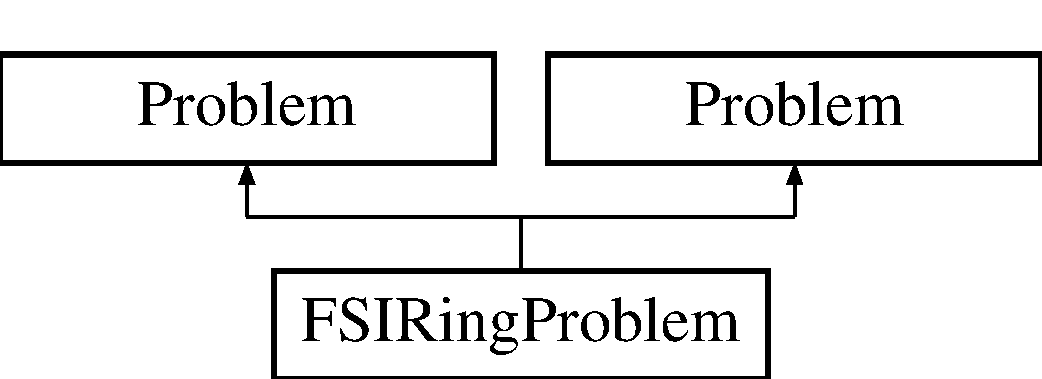
\includegraphics[height=2.000000cm]{classFSIRingProblem}
\end{center}
\end{figure}
\subsection*{Public Member Functions}
\begin{DoxyCompactItemize}
\item 
\hyperlink{classFSIRingProblem_a8f4969c6397bebe8afa2b9285ec908e6}{F\+S\+I\+Ring\+Problem} (const unsigned \&nelement\+\_\+wall, const double \&eps\+\_\+ampl, const double \&pcos\+\_\+initial, const double \&pcos\+\_\+duration)
\item 
void \hyperlink{classFSIRingProblem_a63a3da079b167ccdc288372bee6bdbc3}{actions\+\_\+after\+\_\+newton\+\_\+solve} ()
\begin{DoxyCompactList}\small\item\em Update after solve (empty) \end{DoxyCompactList}\item 
void \hyperlink{classFSIRingProblem_a9fd26120e4e078bca685a5c94482ee12}{actions\+\_\+before\+\_\+newton\+\_\+solve} ()
\begin{DoxyCompactList}\small\item\em Update before solve (empty) \end{DoxyCompactList}\item 
void \hyperlink{classFSIRingProblem_afaf315a9b0feb319cf66b21f959e465e}{actions\+\_\+before\+\_\+newton\+\_\+convergence\+\_\+check} ()
\begin{DoxyCompactList}\small\item\em Update the problem specs before checking Newton convergence. \end{DoxyCompactList}\item 
void \hyperlink{classFSIRingProblem_af4ffa3d628230ef064a84b7c6e6a5fb8}{actions\+\_\+after\+\_\+adapt} ()
\begin{DoxyCompactList}\small\item\em Update the problem specs after adaptation\+: \end{DoxyCompactList}\item 
void \hyperlink{classFSIRingProblem_a686782b9af582b68e55c288e1fe4660e}{doc\+\_\+solution} (const unsigned \&i, Doc\+Info \&doc\+\_\+info, ofstream \&trace\+\_\+file)
\begin{DoxyCompactList}\small\item\em Doc solution\+: Pass number of timestep, i (we append to tracefile after every timestep but do a full doc only at certain intervals), Doc\+Info object and tracefile. \end{DoxyCompactList}\item 
void \hyperlink{classFSIRingProblem_acbb3bc5cd6d16cfee7a2f19a3b984ce7}{dynamic\+\_\+run} ()
\begin{DoxyCompactList}\small\item\em Do dynamic run. \end{DoxyCompactList}\item 
\hyperlink{classFSIRingProblem_a99a92bc3e2713063664277ce535c0af1}{F\+S\+I\+Ring\+Problem} (const unsigned \&nelement\+\_\+wall, const double \&eps\+\_\+ampl, const double \&pcos\+\_\+initial, const double \&pcos\+\_\+duration, const unsigned \&i\+\_\+case)
\item 
void \hyperlink{classFSIRingProblem_a63a3da079b167ccdc288372bee6bdbc3}{actions\+\_\+after\+\_\+newton\+\_\+solve} ()
\begin{DoxyCompactList}\small\item\em Update after solve (empty) \end{DoxyCompactList}\item 
void \hyperlink{classFSIRingProblem_a9fd26120e4e078bca685a5c94482ee12}{actions\+\_\+before\+\_\+newton\+\_\+solve} ()
\begin{DoxyCompactList}\small\item\em Update before solve (empty) \end{DoxyCompactList}\item 
void \hyperlink{classFSIRingProblem_afaf315a9b0feb319cf66b21f959e465e}{actions\+\_\+before\+\_\+newton\+\_\+convergence\+\_\+check} ()
\begin{DoxyCompactList}\small\item\em Update the problem specs before checking Newton convergence. \end{DoxyCompactList}\item 
void \hyperlink{classFSIRingProblem_af4ffa3d628230ef064a84b7c6e6a5fb8}{actions\+\_\+after\+\_\+adapt} ()
\begin{DoxyCompactList}\small\item\em Update the problem specs after adaptation\+: \end{DoxyCompactList}\item 
void \hyperlink{classFSIRingProblem_a6ffbe3f55308ea33cf2cc204062ef4ea}{doc\+\_\+solution} (const unsigned \&i, Doc\+Info \&doc\+\_\+info, ofstream \&trace\+\_\+file, const unsigned \&i\+\_\+case)
\begin{DoxyCompactList}\small\item\em Doc solution\+: Pass number of timestep, i (we append to tracefile after every timestep but do a full doc only at certain intervals), Doc\+Info object and tracefile. \end{DoxyCompactList}\item 
void \hyperlink{classFSIRingProblem_ac679e3984b85ddec7b8c2e8ab4511eac}{dynamic\+\_\+run} (const unsigned \&i\+\_\+case)
\begin{DoxyCompactList}\small\item\em Do dynamic run. \end{DoxyCompactList}\end{DoxyCompactItemize}
\subsection*{Private Types}
\begin{DoxyCompactItemize}
\item 
typedef Algebraic\+Element$<$ Refineable\+Q\+Crouzeix\+Raviart\+Element$<$ 2 $>$ $>$ \hyperlink{classFSIRingProblem_a2ce9ba3122272853bfa6ec3fcf39b78a}{F\+L\+U\+I\+D\+\_\+\+E\+L\+E\+M\+E\+NT}
\begin{DoxyCompactList}\small\item\em There are very few element types that will work for this problem. Rather than passing the element type as a template parameter to the problem, we choose instead to use a typedef to specify the particular element fluid used. \end{DoxyCompactList}\item 
typedef F\+S\+I\+Hermite\+Beam\+Element \hyperlink{classFSIRingProblem_a96528378f3baf6100aeb6b4fe83bc870}{S\+O\+L\+I\+D\+\_\+\+E\+L\+E\+M\+E\+NT}
\begin{DoxyCompactList}\small\item\em Typedef to specify the solid element used. \end{DoxyCompactList}\item 
typedef Algebraic\+Element$<$ Refineable\+Q\+Crouzeix\+Raviart\+Element$<$ 2 $>$ $>$ \hyperlink{classFSIRingProblem_a2ce9ba3122272853bfa6ec3fcf39b78a}{F\+L\+U\+I\+D\+\_\+\+E\+L\+E\+M\+E\+NT}
\begin{DoxyCompactList}\small\item\em There are very few element types that will work for this problem. Rather than passing the element type as a template parameter to the problem, we choose instead to use a typedef to specify the particular element fluid used. \end{DoxyCompactList}\item 
typedef F\+S\+I\+Hermite\+Beam\+Element \hyperlink{classFSIRingProblem_a96528378f3baf6100aeb6b4fe83bc870}{S\+O\+L\+I\+D\+\_\+\+E\+L\+E\+M\+E\+NT}
\begin{DoxyCompactList}\small\item\em Typedef to specify the solid element used. \end{DoxyCompactList}\end{DoxyCompactItemize}
\subsection*{Private Member Functions}
\begin{DoxyCompactItemize}
\item 
void \hyperlink{classFSIRingProblem_a309ea4c79fbae58020d94bf2c2318169}{set\+\_\+initial\+\_\+condition} ()
\begin{DoxyCompactList}\small\item\em Setup initial condition for both domains. \end{DoxyCompactList}\item 
void \hyperlink{classFSIRingProblem_a5f987c1b22dc306cf7d26be7fa74e322}{set\+\_\+wall\+\_\+initial\+\_\+condition} ()
\begin{DoxyCompactList}\small\item\em Setup initial condition for wall. \end{DoxyCompactList}\item 
void \hyperlink{classFSIRingProblem_ad397e4e3b92845240dd6a996856f33e7}{set\+\_\+fluid\+\_\+initial\+\_\+condition} ()
\begin{DoxyCompactList}\small\item\em Setup initial condition for fluid. \end{DoxyCompactList}\item 
void \hyperlink{classFSIRingProblem_a309ea4c79fbae58020d94bf2c2318169}{set\+\_\+initial\+\_\+condition} ()
\begin{DoxyCompactList}\small\item\em Setup initial condition for both domains. \end{DoxyCompactList}\item 
void \hyperlink{classFSIRingProblem_a5f987c1b22dc306cf7d26be7fa74e322}{set\+\_\+wall\+\_\+initial\+\_\+condition} ()
\begin{DoxyCompactList}\small\item\em Setup initial condition for wall. \end{DoxyCompactList}\item 
void \hyperlink{classFSIRingProblem_ad397e4e3b92845240dd6a996856f33e7}{set\+\_\+fluid\+\_\+initial\+\_\+condition} ()
\begin{DoxyCompactList}\small\item\em Setup initial condition for fluid. \end{DoxyCompactList}\end{DoxyCompactItemize}
\subsection*{Private Attributes}
\begin{DoxyCompactItemize}
\item 
\hyperlink{classFSIRingProblem_a96528378f3baf6100aeb6b4fe83bc870}{S\+O\+L\+I\+D\+\_\+\+E\+L\+E\+M\+E\+NT} $\ast$ \hyperlink{classFSIRingProblem_a85d9441c676456c71dffc27500bd0fec}{Doc\+\_\+displacement\+\_\+elem\+\_\+pt}
\begin{DoxyCompactList}\small\item\em Element used for documenting displacement. \end{DoxyCompactList}\item 
One\+D\+Lagrangian\+Mesh$<$ \hyperlink{classFSIRingProblem_a96528378f3baf6100aeb6b4fe83bc870}{S\+O\+L\+I\+D\+\_\+\+E\+L\+E\+M\+E\+NT} $>$ $\ast$ \hyperlink{classFSIRingProblem_a112c5285b6ea49d0e003fc3bdd817332}{Wall\+\_\+mesh\+\_\+pt}
\begin{DoxyCompactList}\small\item\em Pointer to wall mesh. \end{DoxyCompactList}\item 
Algebraic\+Refineable\+Quarter\+Circle\+Sector\+Mesh$<$ \hyperlink{classFSIRingProblem_a2ce9ba3122272853bfa6ec3fcf39b78a}{F\+L\+U\+I\+D\+\_\+\+E\+L\+E\+M\+E\+NT} $>$ $\ast$ \hyperlink{classFSIRingProblem_a33eec722bed7a0b02444c64d3e6c66fe}{Fluid\+\_\+mesh\+\_\+pt}
\begin{DoxyCompactList}\small\item\em Pointer to fluid mesh. \end{DoxyCompactList}\item 
Geom\+Object $\ast$ \hyperlink{classFSIRingProblem_a1c7dfd9d2798fb518403e5ef99f1f69c}{Undef\+\_\+geom\+\_\+pt}
\begin{DoxyCompactList}\small\item\em Pointer to geometric object that represents the undeformed wall shape. \end{DoxyCompactList}\item 
Newmark$<$ 2 $>$ $\ast$ \hyperlink{classFSIRingProblem_a67d7e17b8b0513e793f94fa4357b5784}{Wall\+\_\+time\+\_\+stepper\+\_\+pt}
\begin{DoxyCompactList}\small\item\em Pointer to wall timestepper. \end{DoxyCompactList}\item 
B\+DF$<$ 2 $>$ $\ast$ \hyperlink{classFSIRingProblem_a6abf3345b68a0b4b671758439340138e}{Fluid\+\_\+time\+\_\+stepper\+\_\+pt}
\begin{DoxyCompactList}\small\item\em Pointer to fluid timestepper. \end{DoxyCompactList}\item 
Node $\ast$ \hyperlink{classFSIRingProblem_a2e64e4625ff61633607233d9a6205000}{Veloc\+\_\+trace\+\_\+node\+\_\+pt}
\begin{DoxyCompactList}\small\item\em Pointer to node on coarsest mesh on which velocity is traced. \end{DoxyCompactList}\item 
double \hyperlink{classFSIRingProblem_a6e14af107a8f5b5a5254a55f0707ff4c}{Eps\+\_\+ampl}
\begin{DoxyCompactList}\small\item\em Amplitude of initial deformation. \end{DoxyCompactList}\item 
double \hyperlink{classFSIRingProblem_a109eb6d9804264294357d6b76aa50ab6}{Pcos\+\_\+initial}
\begin{DoxyCompactList}\small\item\em Initial pcos. \end{DoxyCompactList}\item 
double \hyperlink{classFSIRingProblem_a90ff979880dbecb47f8830f4217eb17f}{Pcos\+\_\+duration}
\begin{DoxyCompactList}\small\item\em Duration of initial pcos. \end{DoxyCompactList}\end{DoxyCompactItemize}


\subsection{Detailed Description}
F\+SI Ring problem\+: a fluid-\/structure interaction problem in which a viscous fluid bounded by an initially circular beam is set into motion by a small sinusoidal perturbation of the beam (the domain boundary). 

Definition at line 144 of file fsi\+\_\+osc\+\_\+ring.\+cc.



\subsection{Member Typedef Documentation}
\mbox{\Hypertarget{classFSIRingProblem_a2ce9ba3122272853bfa6ec3fcf39b78a}\label{classFSIRingProblem_a2ce9ba3122272853bfa6ec3fcf39b78a}} 
\index{F\+S\+I\+Ring\+Problem@{F\+S\+I\+Ring\+Problem}!F\+L\+U\+I\+D\+\_\+\+E\+L\+E\+M\+E\+NT@{F\+L\+U\+I\+D\+\_\+\+E\+L\+E\+M\+E\+NT}}
\index{F\+L\+U\+I\+D\+\_\+\+E\+L\+E\+M\+E\+NT@{F\+L\+U\+I\+D\+\_\+\+E\+L\+E\+M\+E\+NT}!F\+S\+I\+Ring\+Problem@{F\+S\+I\+Ring\+Problem}}
\subsubsection{\texorpdfstring{F\+L\+U\+I\+D\+\_\+\+E\+L\+E\+M\+E\+NT}{FLUID\_ELEMENT}\hspace{0.1cm}{\footnotesize\ttfamily [1/2]}}
{\footnotesize\ttfamily typedef Algebraic\+Element$<$Refineable\+Q\+Crouzeix\+Raviart\+Element$<$2$>$ $>$ \hyperlink{classFSIRingProblem_a2ce9ba3122272853bfa6ec3fcf39b78a}{F\+S\+I\+Ring\+Problem\+::\+F\+L\+U\+I\+D\+\_\+\+E\+L\+E\+M\+E\+NT}\hspace{0.3cm}{\ttfamily [private]}}



There are very few element types that will work for this problem. Rather than passing the element type as a template parameter to the problem, we choose instead to use a typedef to specify the particular element fluid used. 



Definition at line 150 of file fsi\+\_\+osc\+\_\+ring.\+cc.

\mbox{\Hypertarget{classFSIRingProblem_a2ce9ba3122272853bfa6ec3fcf39b78a}\label{classFSIRingProblem_a2ce9ba3122272853bfa6ec3fcf39b78a}} 
\index{F\+S\+I\+Ring\+Problem@{F\+S\+I\+Ring\+Problem}!F\+L\+U\+I\+D\+\_\+\+E\+L\+E\+M\+E\+NT@{F\+L\+U\+I\+D\+\_\+\+E\+L\+E\+M\+E\+NT}}
\index{F\+L\+U\+I\+D\+\_\+\+E\+L\+E\+M\+E\+NT@{F\+L\+U\+I\+D\+\_\+\+E\+L\+E\+M\+E\+NT}!F\+S\+I\+Ring\+Problem@{F\+S\+I\+Ring\+Problem}}
\subsubsection{\texorpdfstring{F\+L\+U\+I\+D\+\_\+\+E\+L\+E\+M\+E\+NT}{FLUID\_ELEMENT}\hspace{0.1cm}{\footnotesize\ttfamily [2/2]}}
{\footnotesize\ttfamily typedef Algebraic\+Element$<$Refineable\+Q\+Crouzeix\+Raviart\+Element$<$2$>$ $>$ \hyperlink{classFSIRingProblem_a2ce9ba3122272853bfa6ec3fcf39b78a}{F\+S\+I\+Ring\+Problem\+::\+F\+L\+U\+I\+D\+\_\+\+E\+L\+E\+M\+E\+NT}\hspace{0.3cm}{\ttfamily [private]}}



There are very few element types that will work for this problem. Rather than passing the element type as a template parameter to the problem, we choose instead to use a typedef to specify the particular element fluid used. 



Definition at line 150 of file fsi\+\_\+osc\+\_\+ring\+\_\+compare\+\_\+jacs.\+cc.

\mbox{\Hypertarget{classFSIRingProblem_a96528378f3baf6100aeb6b4fe83bc870}\label{classFSIRingProblem_a96528378f3baf6100aeb6b4fe83bc870}} 
\index{F\+S\+I\+Ring\+Problem@{F\+S\+I\+Ring\+Problem}!S\+O\+L\+I\+D\+\_\+\+E\+L\+E\+M\+E\+NT@{S\+O\+L\+I\+D\+\_\+\+E\+L\+E\+M\+E\+NT}}
\index{S\+O\+L\+I\+D\+\_\+\+E\+L\+E\+M\+E\+NT@{S\+O\+L\+I\+D\+\_\+\+E\+L\+E\+M\+E\+NT}!F\+S\+I\+Ring\+Problem@{F\+S\+I\+Ring\+Problem}}
\subsubsection{\texorpdfstring{S\+O\+L\+I\+D\+\_\+\+E\+L\+E\+M\+E\+NT}{SOLID\_ELEMENT}\hspace{0.1cm}{\footnotesize\ttfamily [1/2]}}
{\footnotesize\ttfamily typedef F\+S\+I\+Hermite\+Beam\+Element \hyperlink{classFSIRingProblem_a96528378f3baf6100aeb6b4fe83bc870}{F\+S\+I\+Ring\+Problem\+::\+S\+O\+L\+I\+D\+\_\+\+E\+L\+E\+M\+E\+NT}\hspace{0.3cm}{\ttfamily [private]}}



Typedef to specify the solid element used. 



Definition at line 153 of file fsi\+\_\+osc\+\_\+ring\+\_\+compare\+\_\+jacs.\+cc.

\mbox{\Hypertarget{classFSIRingProblem_a96528378f3baf6100aeb6b4fe83bc870}\label{classFSIRingProblem_a96528378f3baf6100aeb6b4fe83bc870}} 
\index{F\+S\+I\+Ring\+Problem@{F\+S\+I\+Ring\+Problem}!S\+O\+L\+I\+D\+\_\+\+E\+L\+E\+M\+E\+NT@{S\+O\+L\+I\+D\+\_\+\+E\+L\+E\+M\+E\+NT}}
\index{S\+O\+L\+I\+D\+\_\+\+E\+L\+E\+M\+E\+NT@{S\+O\+L\+I\+D\+\_\+\+E\+L\+E\+M\+E\+NT}!F\+S\+I\+Ring\+Problem@{F\+S\+I\+Ring\+Problem}}
\subsubsection{\texorpdfstring{S\+O\+L\+I\+D\+\_\+\+E\+L\+E\+M\+E\+NT}{SOLID\_ELEMENT}\hspace{0.1cm}{\footnotesize\ttfamily [2/2]}}
{\footnotesize\ttfamily typedef F\+S\+I\+Hermite\+Beam\+Element \hyperlink{classFSIRingProblem_a96528378f3baf6100aeb6b4fe83bc870}{F\+S\+I\+Ring\+Problem\+::\+S\+O\+L\+I\+D\+\_\+\+E\+L\+E\+M\+E\+NT}\hspace{0.3cm}{\ttfamily [private]}}



Typedef to specify the solid element used. 



Definition at line 153 of file fsi\+\_\+osc\+\_\+ring.\+cc.



\subsection{Constructor \& Destructor Documentation}
\mbox{\Hypertarget{classFSIRingProblem_a8f4969c6397bebe8afa2b9285ec908e6}\label{classFSIRingProblem_a8f4969c6397bebe8afa2b9285ec908e6}} 
\index{F\+S\+I\+Ring\+Problem@{F\+S\+I\+Ring\+Problem}!F\+S\+I\+Ring\+Problem@{F\+S\+I\+Ring\+Problem}}
\index{F\+S\+I\+Ring\+Problem@{F\+S\+I\+Ring\+Problem}!F\+S\+I\+Ring\+Problem@{F\+S\+I\+Ring\+Problem}}
\subsubsection{\texorpdfstring{F\+S\+I\+Ring\+Problem()}{FSIRingProblem()}\hspace{0.1cm}{\footnotesize\ttfamily [1/2]}}
{\footnotesize\ttfamily F\+S\+I\+Ring\+Problem\+::\+F\+S\+I\+Ring\+Problem (\begin{DoxyParamCaption}\item[{const unsigned \&}]{N,  }\item[{const double \&}]{eps\+\_\+ampl,  }\item[{const double \&}]{pcos\+\_\+initial,  }\item[{const double \&}]{pcos\+\_\+duration }\end{DoxyParamCaption})}

Constructor\+: Number of elements in wall mesh, amplitude of the initial wall deformation, amplitude of pcos perturbation and its duration.

Constructor for F\+SI ring problem. Pass number of wall elements and length of wall (in Lagrangian coordinates) amplitude of initial deformation, pcos perturbation and duration. 

Definition at line 434 of file fsi\+\_\+osc\+\_\+ring.\+cc.



References Doc\+\_\+displacement\+\_\+elem\+\_\+pt, Fluid\+\_\+mesh\+\_\+pt, Fluid\+\_\+time\+\_\+stepper\+\_\+pt, Global\+\_\+\+Physical\+\_\+\+Variables\+::H, Global\+\_\+\+Physical\+\_\+\+Variables\+::\+Lambda\+\_\+sq, oomph\+::\+Sarah\+B\+L\+::N, Global\+\_\+\+Physical\+\_\+\+Variables\+::pcos\+\_\+load(), Global\+\_\+\+Physical\+\_\+\+Variables\+::Q, Global\+\_\+\+Physical\+\_\+\+Variables\+::\+Re, Global\+\_\+\+Physical\+\_\+\+Variables\+::\+Re\+St, Undef\+\_\+geom\+\_\+pt, Veloc\+\_\+trace\+\_\+node\+\_\+pt, Wall\+\_\+mesh\+\_\+pt, and Wall\+\_\+time\+\_\+stepper\+\_\+pt.

\mbox{\Hypertarget{classFSIRingProblem_a99a92bc3e2713063664277ce535c0af1}\label{classFSIRingProblem_a99a92bc3e2713063664277ce535c0af1}} 
\index{F\+S\+I\+Ring\+Problem@{F\+S\+I\+Ring\+Problem}!F\+S\+I\+Ring\+Problem@{F\+S\+I\+Ring\+Problem}}
\index{F\+S\+I\+Ring\+Problem@{F\+S\+I\+Ring\+Problem}!F\+S\+I\+Ring\+Problem@{F\+S\+I\+Ring\+Problem}}
\subsubsection{\texorpdfstring{F\+S\+I\+Ring\+Problem()}{FSIRingProblem()}\hspace{0.1cm}{\footnotesize\ttfamily [2/2]}}
{\footnotesize\ttfamily F\+S\+I\+Ring\+Problem\+::\+F\+S\+I\+Ring\+Problem (\begin{DoxyParamCaption}\item[{const unsigned \&}]{N,  }\item[{const double \&}]{eps\+\_\+ampl,  }\item[{const double \&}]{pcos\+\_\+initial,  }\item[{const double \&}]{pcos\+\_\+duration,  }\item[{const unsigned \&}]{i\+\_\+case }\end{DoxyParamCaption})}

Constructor\+: Number of elements in wall mesh, amplitude of the initial wall deformation, amplitude of pcos perturbation and its duration.

Constructor for F\+SI ring problem. Pass number of wall elements and length of wall (in Lagrangian coordinates) amplitude of initial deformation, pcos perturbation and duration. 

Definition at line 435 of file fsi\+\_\+osc\+\_\+ring\+\_\+compare\+\_\+jacs.\+cc.



References Doc\+\_\+displacement\+\_\+elem\+\_\+pt, Fluid\+\_\+mesh\+\_\+pt, Fluid\+\_\+time\+\_\+stepper\+\_\+pt, Global\+\_\+\+Physical\+\_\+\+Variables\+::H, Global\+\_\+\+Physical\+\_\+\+Variables\+::\+Lambda\+\_\+sq, oomph\+::\+Sarah\+B\+L\+::N, Global\+\_\+\+Physical\+\_\+\+Variables\+::pcos\+\_\+load(), Global\+\_\+\+Physical\+\_\+\+Variables\+::Q, Global\+\_\+\+Physical\+\_\+\+Variables\+::\+Re, Global\+\_\+\+Physical\+\_\+\+Variables\+::\+Re\+St, Undef\+\_\+geom\+\_\+pt, Veloc\+\_\+trace\+\_\+node\+\_\+pt, Wall\+\_\+mesh\+\_\+pt, and Wall\+\_\+time\+\_\+stepper\+\_\+pt.



\subsection{Member Function Documentation}
\mbox{\Hypertarget{classFSIRingProblem_af4ffa3d628230ef064a84b7c6e6a5fb8}\label{classFSIRingProblem_af4ffa3d628230ef064a84b7c6e6a5fb8}} 
\index{F\+S\+I\+Ring\+Problem@{F\+S\+I\+Ring\+Problem}!actions\+\_\+after\+\_\+adapt@{actions\+\_\+after\+\_\+adapt}}
\index{actions\+\_\+after\+\_\+adapt@{actions\+\_\+after\+\_\+adapt}!F\+S\+I\+Ring\+Problem@{F\+S\+I\+Ring\+Problem}}
\subsubsection{\texorpdfstring{actions\+\_\+after\+\_\+adapt()}{actions\_after\_adapt()}\hspace{0.1cm}{\footnotesize\ttfamily [1/2]}}
{\footnotesize\ttfamily void F\+S\+I\+Ring\+Problem\+::actions\+\_\+after\+\_\+adapt (\begin{DoxyParamCaption}{ }\end{DoxyParamCaption})\hspace{0.3cm}{\ttfamily [inline]}}



Update the problem specs after adaptation\+: 



Definition at line 179 of file fsi\+\_\+osc\+\_\+ring.\+cc.

\mbox{\Hypertarget{classFSIRingProblem_af4ffa3d628230ef064a84b7c6e6a5fb8}\label{classFSIRingProblem_af4ffa3d628230ef064a84b7c6e6a5fb8}} 
\index{F\+S\+I\+Ring\+Problem@{F\+S\+I\+Ring\+Problem}!actions\+\_\+after\+\_\+adapt@{actions\+\_\+after\+\_\+adapt}}
\index{actions\+\_\+after\+\_\+adapt@{actions\+\_\+after\+\_\+adapt}!F\+S\+I\+Ring\+Problem@{F\+S\+I\+Ring\+Problem}}
\subsubsection{\texorpdfstring{actions\+\_\+after\+\_\+adapt()}{actions\_after\_adapt()}\hspace{0.1cm}{\footnotesize\ttfamily [2/2]}}
{\footnotesize\ttfamily void F\+S\+I\+Ring\+Problem\+::actions\+\_\+after\+\_\+adapt (\begin{DoxyParamCaption}{ }\end{DoxyParamCaption})\hspace{0.3cm}{\ttfamily [inline]}}



Update the problem specs after adaptation\+: 



Definition at line 179 of file fsi\+\_\+osc\+\_\+ring\+\_\+compare\+\_\+jacs.\+cc.



References Global\+\_\+\+Physical\+\_\+\+Variables\+::H, set\+\_\+fluid\+\_\+initial\+\_\+condition(), set\+\_\+initial\+\_\+condition(), and set\+\_\+wall\+\_\+initial\+\_\+condition().

\mbox{\Hypertarget{classFSIRingProblem_a63a3da079b167ccdc288372bee6bdbc3}\label{classFSIRingProblem_a63a3da079b167ccdc288372bee6bdbc3}} 
\index{F\+S\+I\+Ring\+Problem@{F\+S\+I\+Ring\+Problem}!actions\+\_\+after\+\_\+newton\+\_\+solve@{actions\+\_\+after\+\_\+newton\+\_\+solve}}
\index{actions\+\_\+after\+\_\+newton\+\_\+solve@{actions\+\_\+after\+\_\+newton\+\_\+solve}!F\+S\+I\+Ring\+Problem@{F\+S\+I\+Ring\+Problem}}
\subsubsection{\texorpdfstring{actions\+\_\+after\+\_\+newton\+\_\+solve()}{actions\_after\_newton\_solve()}\hspace{0.1cm}{\footnotesize\ttfamily [1/2]}}
{\footnotesize\ttfamily void F\+S\+I\+Ring\+Problem\+::actions\+\_\+after\+\_\+newton\+\_\+solve (\begin{DoxyParamCaption}{ }\end{DoxyParamCaption})\hspace{0.3cm}{\ttfamily [inline]}}



Update after solve (empty) 



Definition at line 164 of file fsi\+\_\+osc\+\_\+ring.\+cc.

\mbox{\Hypertarget{classFSIRingProblem_a63a3da079b167ccdc288372bee6bdbc3}\label{classFSIRingProblem_a63a3da079b167ccdc288372bee6bdbc3}} 
\index{F\+S\+I\+Ring\+Problem@{F\+S\+I\+Ring\+Problem}!actions\+\_\+after\+\_\+newton\+\_\+solve@{actions\+\_\+after\+\_\+newton\+\_\+solve}}
\index{actions\+\_\+after\+\_\+newton\+\_\+solve@{actions\+\_\+after\+\_\+newton\+\_\+solve}!F\+S\+I\+Ring\+Problem@{F\+S\+I\+Ring\+Problem}}
\subsubsection{\texorpdfstring{actions\+\_\+after\+\_\+newton\+\_\+solve()}{actions\_after\_newton\_solve()}\hspace{0.1cm}{\footnotesize\ttfamily [2/2]}}
{\footnotesize\ttfamily void F\+S\+I\+Ring\+Problem\+::actions\+\_\+after\+\_\+newton\+\_\+solve (\begin{DoxyParamCaption}{ }\end{DoxyParamCaption})\hspace{0.3cm}{\ttfamily [inline]}}



Update after solve (empty) 



Definition at line 164 of file fsi\+\_\+osc\+\_\+ring\+\_\+compare\+\_\+jacs.\+cc.

\mbox{\Hypertarget{classFSIRingProblem_afaf315a9b0feb319cf66b21f959e465e}\label{classFSIRingProblem_afaf315a9b0feb319cf66b21f959e465e}} 
\index{F\+S\+I\+Ring\+Problem@{F\+S\+I\+Ring\+Problem}!actions\+\_\+before\+\_\+newton\+\_\+convergence\+\_\+check@{actions\+\_\+before\+\_\+newton\+\_\+convergence\+\_\+check}}
\index{actions\+\_\+before\+\_\+newton\+\_\+convergence\+\_\+check@{actions\+\_\+before\+\_\+newton\+\_\+convergence\+\_\+check}!F\+S\+I\+Ring\+Problem@{F\+S\+I\+Ring\+Problem}}
\subsubsection{\texorpdfstring{actions\+\_\+before\+\_\+newton\+\_\+convergence\+\_\+check()}{actions\_before\_newton\_convergence\_check()}\hspace{0.1cm}{\footnotesize\ttfamily [1/2]}}
{\footnotesize\ttfamily void F\+S\+I\+Ring\+Problem\+::actions\+\_\+before\+\_\+newton\+\_\+convergence\+\_\+check (\begin{DoxyParamCaption}{ }\end{DoxyParamCaption})\hspace{0.3cm}{\ttfamily [inline]}}



Update the problem specs before checking Newton convergence. 



Definition at line 171 of file fsi\+\_\+osc\+\_\+ring.\+cc.

\mbox{\Hypertarget{classFSIRingProblem_afaf315a9b0feb319cf66b21f959e465e}\label{classFSIRingProblem_afaf315a9b0feb319cf66b21f959e465e}} 
\index{F\+S\+I\+Ring\+Problem@{F\+S\+I\+Ring\+Problem}!actions\+\_\+before\+\_\+newton\+\_\+convergence\+\_\+check@{actions\+\_\+before\+\_\+newton\+\_\+convergence\+\_\+check}}
\index{actions\+\_\+before\+\_\+newton\+\_\+convergence\+\_\+check@{actions\+\_\+before\+\_\+newton\+\_\+convergence\+\_\+check}!F\+S\+I\+Ring\+Problem@{F\+S\+I\+Ring\+Problem}}
\subsubsection{\texorpdfstring{actions\+\_\+before\+\_\+newton\+\_\+convergence\+\_\+check()}{actions\_before\_newton\_convergence\_check()}\hspace{0.1cm}{\footnotesize\ttfamily [2/2]}}
{\footnotesize\ttfamily void F\+S\+I\+Ring\+Problem\+::actions\+\_\+before\+\_\+newton\+\_\+convergence\+\_\+check (\begin{DoxyParamCaption}{ }\end{DoxyParamCaption})\hspace{0.3cm}{\ttfamily [inline]}}



Update the problem specs before checking Newton convergence. 



Definition at line 171 of file fsi\+\_\+osc\+\_\+ring\+\_\+compare\+\_\+jacs.\+cc.

\mbox{\Hypertarget{classFSIRingProblem_a9fd26120e4e078bca685a5c94482ee12}\label{classFSIRingProblem_a9fd26120e4e078bca685a5c94482ee12}} 
\index{F\+S\+I\+Ring\+Problem@{F\+S\+I\+Ring\+Problem}!actions\+\_\+before\+\_\+newton\+\_\+solve@{actions\+\_\+before\+\_\+newton\+\_\+solve}}
\index{actions\+\_\+before\+\_\+newton\+\_\+solve@{actions\+\_\+before\+\_\+newton\+\_\+solve}!F\+S\+I\+Ring\+Problem@{F\+S\+I\+Ring\+Problem}}
\subsubsection{\texorpdfstring{actions\+\_\+before\+\_\+newton\+\_\+solve()}{actions\_before\_newton\_solve()}\hspace{0.1cm}{\footnotesize\ttfamily [1/2]}}
{\footnotesize\ttfamily void F\+S\+I\+Ring\+Problem\+::actions\+\_\+before\+\_\+newton\+\_\+solve (\begin{DoxyParamCaption}{ }\end{DoxyParamCaption})\hspace{0.3cm}{\ttfamily [inline]}}



Update before solve (empty) 



Definition at line 167 of file fsi\+\_\+osc\+\_\+ring.\+cc.

\mbox{\Hypertarget{classFSIRingProblem_a9fd26120e4e078bca685a5c94482ee12}\label{classFSIRingProblem_a9fd26120e4e078bca685a5c94482ee12}} 
\index{F\+S\+I\+Ring\+Problem@{F\+S\+I\+Ring\+Problem}!actions\+\_\+before\+\_\+newton\+\_\+solve@{actions\+\_\+before\+\_\+newton\+\_\+solve}}
\index{actions\+\_\+before\+\_\+newton\+\_\+solve@{actions\+\_\+before\+\_\+newton\+\_\+solve}!F\+S\+I\+Ring\+Problem@{F\+S\+I\+Ring\+Problem}}
\subsubsection{\texorpdfstring{actions\+\_\+before\+\_\+newton\+\_\+solve()}{actions\_before\_newton\_solve()}\hspace{0.1cm}{\footnotesize\ttfamily [2/2]}}
{\footnotesize\ttfamily void F\+S\+I\+Ring\+Problem\+::actions\+\_\+before\+\_\+newton\+\_\+solve (\begin{DoxyParamCaption}{ }\end{DoxyParamCaption})\hspace{0.3cm}{\ttfamily [inline]}}



Update before solve (empty) 



Definition at line 167 of file fsi\+\_\+osc\+\_\+ring\+\_\+compare\+\_\+jacs.\+cc.

\mbox{\Hypertarget{classFSIRingProblem_a686782b9af582b68e55c288e1fe4660e}\label{classFSIRingProblem_a686782b9af582b68e55c288e1fe4660e}} 
\index{F\+S\+I\+Ring\+Problem@{F\+S\+I\+Ring\+Problem}!doc\+\_\+solution@{doc\+\_\+solution}}
\index{doc\+\_\+solution@{doc\+\_\+solution}!F\+S\+I\+Ring\+Problem@{F\+S\+I\+Ring\+Problem}}
\subsubsection{\texorpdfstring{doc\+\_\+solution()}{doc\_solution()}\hspace{0.1cm}{\footnotesize\ttfamily [1/2]}}
{\footnotesize\ttfamily void F\+S\+I\+Ring\+Problem\+::doc\+\_\+solution (\begin{DoxyParamCaption}\item[{const unsigned \&}]{i,  }\item[{Doc\+Info \&}]{doc\+\_\+info,  }\item[{ofstream \&}]{trace\+\_\+file }\end{DoxyParamCaption})}



Doc solution\+: Pass number of timestep, i (we append to tracefile after every timestep but do a full doc only at certain intervals), Doc\+Info object and tracefile. 

Document solution\+: Pass number of timestep, i; we append to trace file at every timestep and do a full doc only after a certain number of steps. Output the solution using 5x5 plot points 

Definition at line 356 of file fsi\+\_\+osc\+\_\+ring.\+cc.



Referenced by dynamic\+\_\+run().

\mbox{\Hypertarget{classFSIRingProblem_a6ffbe3f55308ea33cf2cc204062ef4ea}\label{classFSIRingProblem_a6ffbe3f55308ea33cf2cc204062ef4ea}} 
\index{F\+S\+I\+Ring\+Problem@{F\+S\+I\+Ring\+Problem}!doc\+\_\+solution@{doc\+\_\+solution}}
\index{doc\+\_\+solution@{doc\+\_\+solution}!F\+S\+I\+Ring\+Problem@{F\+S\+I\+Ring\+Problem}}
\subsubsection{\texorpdfstring{doc\+\_\+solution()}{doc\_solution()}\hspace{0.1cm}{\footnotesize\ttfamily [2/2]}}
{\footnotesize\ttfamily void F\+S\+I\+Ring\+Problem\+::doc\+\_\+solution (\begin{DoxyParamCaption}\item[{const unsigned \&}]{i,  }\item[{Doc\+Info \&}]{doc\+\_\+info,  }\item[{ofstream \&}]{trace\+\_\+file,  }\item[{const unsigned \&}]{i\+\_\+case }\end{DoxyParamCaption})}



Doc solution\+: Pass number of timestep, i (we append to tracefile after every timestep but do a full doc only at certain intervals), Doc\+Info object and tracefile. 

Document solution\+: Pass number of timestep, i; we append to trace file at every timestep and do a full doc only after a certain number of steps. Output the solution using 5x5 plot points 

Definition at line 357 of file fsi\+\_\+osc\+\_\+ring\+\_\+compare\+\_\+jacs.\+cc.

\mbox{\Hypertarget{classFSIRingProblem_acbb3bc5cd6d16cfee7a2f19a3b984ce7}\label{classFSIRingProblem_acbb3bc5cd6d16cfee7a2f19a3b984ce7}} 
\index{F\+S\+I\+Ring\+Problem@{F\+S\+I\+Ring\+Problem}!dynamic\+\_\+run@{dynamic\+\_\+run}}
\index{dynamic\+\_\+run@{dynamic\+\_\+run}!F\+S\+I\+Ring\+Problem@{F\+S\+I\+Ring\+Problem}}
\subsubsection{\texorpdfstring{dynamic\+\_\+run()}{dynamic\_run()}\hspace{0.1cm}{\footnotesize\ttfamily [1/2]}}
{\footnotesize\ttfamily void F\+S\+I\+Ring\+Problem\+::dynamic\+\_\+run (\begin{DoxyParamCaption}{ }\end{DoxyParamCaption})}



Do dynamic run. 

Solver loop to perform unsteady run. Label for output

Perturbation pressure

Switch off perturbation pressure 

Definition at line 660 of file fsi\+\_\+osc\+\_\+ring.\+cc.



References Global\+\_\+\+Physical\+\_\+\+Variables\+::\+Alpha\+\_\+sq, Global\+\_\+\+Physical\+\_\+\+Variables\+::\+Density\+\_\+ratio, doc\+\_\+solution(), Fluid\+\_\+mesh\+\_\+pt, Global\+\_\+\+Physical\+\_\+\+Variables\+::H, Global\+\_\+\+Physical\+\_\+\+Variables\+::\+Pcos, Pcos\+\_\+duration, Pcos\+\_\+initial, Global\+\_\+\+Physical\+\_\+\+Variables\+::\+Pext, set\+\_\+initial\+\_\+condition(), and Global\+\_\+\+Physical\+\_\+\+Variables\+::set\+\_\+params().



Referenced by main().

\mbox{\Hypertarget{classFSIRingProblem_ac679e3984b85ddec7b8c2e8ab4511eac}\label{classFSIRingProblem_ac679e3984b85ddec7b8c2e8ab4511eac}} 
\index{F\+S\+I\+Ring\+Problem@{F\+S\+I\+Ring\+Problem}!dynamic\+\_\+run@{dynamic\+\_\+run}}
\index{dynamic\+\_\+run@{dynamic\+\_\+run}!F\+S\+I\+Ring\+Problem@{F\+S\+I\+Ring\+Problem}}
\subsubsection{\texorpdfstring{dynamic\+\_\+run()}{dynamic\_run()}\hspace{0.1cm}{\footnotesize\ttfamily [2/2]}}
{\footnotesize\ttfamily void F\+S\+I\+Ring\+Problem\+::dynamic\+\_\+run (\begin{DoxyParamCaption}\item[{const unsigned \&}]{i\+\_\+case }\end{DoxyParamCaption})}



Do dynamic run. 

Solver loop to perform unsteady run. Label for output

Perturbation pressure

Switch off perturbation pressure 

Definition at line 703 of file fsi\+\_\+osc\+\_\+ring\+\_\+compare\+\_\+jacs.\+cc.



References doc\+\_\+solution(), Fluid\+\_\+mesh\+\_\+pt, Pcos\+\_\+duration, Pcos\+\_\+initial, set\+\_\+initial\+\_\+condition(), and Global\+\_\+\+Physical\+\_\+\+Variables\+::set\+\_\+params().

\mbox{\Hypertarget{classFSIRingProblem_ad397e4e3b92845240dd6a996856f33e7}\label{classFSIRingProblem_ad397e4e3b92845240dd6a996856f33e7}} 
\index{F\+S\+I\+Ring\+Problem@{F\+S\+I\+Ring\+Problem}!set\+\_\+fluid\+\_\+initial\+\_\+condition@{set\+\_\+fluid\+\_\+initial\+\_\+condition}}
\index{set\+\_\+fluid\+\_\+initial\+\_\+condition@{set\+\_\+fluid\+\_\+initial\+\_\+condition}!F\+S\+I\+Ring\+Problem@{F\+S\+I\+Ring\+Problem}}
\subsubsection{\texorpdfstring{set\+\_\+fluid\+\_\+initial\+\_\+condition()}{set\_fluid\_initial\_condition()}\hspace{0.1cm}{\footnotesize\ttfamily [1/2]}}
{\footnotesize\ttfamily void F\+S\+I\+Ring\+Problem\+::set\+\_\+fluid\+\_\+initial\+\_\+condition (\begin{DoxyParamCaption}{ }\end{DoxyParamCaption})\hspace{0.3cm}{\ttfamily [private]}}



Setup initial condition for fluid. 

Setup initial condition for fluid\+: Impulsive start. 

Definition at line 283 of file fsi\+\_\+osc\+\_\+ring.\+cc.



Referenced by actions\+\_\+after\+\_\+adapt().

\mbox{\Hypertarget{classFSIRingProblem_ad397e4e3b92845240dd6a996856f33e7}\label{classFSIRingProblem_ad397e4e3b92845240dd6a996856f33e7}} 
\index{F\+S\+I\+Ring\+Problem@{F\+S\+I\+Ring\+Problem}!set\+\_\+fluid\+\_\+initial\+\_\+condition@{set\+\_\+fluid\+\_\+initial\+\_\+condition}}
\index{set\+\_\+fluid\+\_\+initial\+\_\+condition@{set\+\_\+fluid\+\_\+initial\+\_\+condition}!F\+S\+I\+Ring\+Problem@{F\+S\+I\+Ring\+Problem}}
\subsubsection{\texorpdfstring{set\+\_\+fluid\+\_\+initial\+\_\+condition()}{set\_fluid\_initial\_condition()}\hspace{0.1cm}{\footnotesize\ttfamily [2/2]}}
{\footnotesize\ttfamily void F\+S\+I\+Ring\+Problem\+::set\+\_\+fluid\+\_\+initial\+\_\+condition (\begin{DoxyParamCaption}{ }\end{DoxyParamCaption})\hspace{0.3cm}{\ttfamily [private]}}



Setup initial condition for fluid. 

\mbox{\Hypertarget{classFSIRingProblem_a309ea4c79fbae58020d94bf2c2318169}\label{classFSIRingProblem_a309ea4c79fbae58020d94bf2c2318169}} 
\index{F\+S\+I\+Ring\+Problem@{F\+S\+I\+Ring\+Problem}!set\+\_\+initial\+\_\+condition@{set\+\_\+initial\+\_\+condition}}
\index{set\+\_\+initial\+\_\+condition@{set\+\_\+initial\+\_\+condition}!F\+S\+I\+Ring\+Problem@{F\+S\+I\+Ring\+Problem}}
\subsubsection{\texorpdfstring{set\+\_\+initial\+\_\+condition()}{set\_initial\_condition()}\hspace{0.1cm}{\footnotesize\ttfamily [1/2]}}
{\footnotesize\ttfamily void F\+S\+I\+Ring\+Problem\+::set\+\_\+initial\+\_\+condition (\begin{DoxyParamCaption}{ }\end{DoxyParamCaption})\hspace{0.3cm}{\ttfamily [private]}}



Setup initial condition for both domains. 

Setup initial condition\+: When we\textquotesingle{}re done here, all variables represent the state at the initial time. 

Definition at line 268 of file fsi\+\_\+osc\+\_\+ring.\+cc.



Referenced by actions\+\_\+after\+\_\+adapt(), and dynamic\+\_\+run().

\mbox{\Hypertarget{classFSIRingProblem_a309ea4c79fbae58020d94bf2c2318169}\label{classFSIRingProblem_a309ea4c79fbae58020d94bf2c2318169}} 
\index{F\+S\+I\+Ring\+Problem@{F\+S\+I\+Ring\+Problem}!set\+\_\+initial\+\_\+condition@{set\+\_\+initial\+\_\+condition}}
\index{set\+\_\+initial\+\_\+condition@{set\+\_\+initial\+\_\+condition}!F\+S\+I\+Ring\+Problem@{F\+S\+I\+Ring\+Problem}}
\subsubsection{\texorpdfstring{set\+\_\+initial\+\_\+condition()}{set\_initial\_condition()}\hspace{0.1cm}{\footnotesize\ttfamily [2/2]}}
{\footnotesize\ttfamily void F\+S\+I\+Ring\+Problem\+::set\+\_\+initial\+\_\+condition (\begin{DoxyParamCaption}{ }\end{DoxyParamCaption})\hspace{0.3cm}{\ttfamily [private]}}



Setup initial condition for both domains. 

\mbox{\Hypertarget{classFSIRingProblem_a5f987c1b22dc306cf7d26be7fa74e322}\label{classFSIRingProblem_a5f987c1b22dc306cf7d26be7fa74e322}} 
\index{F\+S\+I\+Ring\+Problem@{F\+S\+I\+Ring\+Problem}!set\+\_\+wall\+\_\+initial\+\_\+condition@{set\+\_\+wall\+\_\+initial\+\_\+condition}}
\index{set\+\_\+wall\+\_\+initial\+\_\+condition@{set\+\_\+wall\+\_\+initial\+\_\+condition}!F\+S\+I\+Ring\+Problem@{F\+S\+I\+Ring\+Problem}}
\subsubsection{\texorpdfstring{set\+\_\+wall\+\_\+initial\+\_\+condition()}{set\_wall\_initial\_condition()}\hspace{0.1cm}{\footnotesize\ttfamily [1/2]}}
{\footnotesize\ttfamily void F\+S\+I\+Ring\+Problem\+::set\+\_\+wall\+\_\+initial\+\_\+condition (\begin{DoxyParamCaption}{ }\end{DoxyParamCaption})\hspace{0.3cm}{\ttfamily [private]}}



Setup initial condition for wall. 

Setup initial condition\+: Impulsive start either from deformed or undeformed wall shape. 

Definition at line 322 of file fsi\+\_\+osc\+\_\+ring.\+cc.



References Global\+\_\+\+Physical\+\_\+\+Variables\+::H.



Referenced by actions\+\_\+after\+\_\+adapt().

\mbox{\Hypertarget{classFSIRingProblem_a5f987c1b22dc306cf7d26be7fa74e322}\label{classFSIRingProblem_a5f987c1b22dc306cf7d26be7fa74e322}} 
\index{F\+S\+I\+Ring\+Problem@{F\+S\+I\+Ring\+Problem}!set\+\_\+wall\+\_\+initial\+\_\+condition@{set\+\_\+wall\+\_\+initial\+\_\+condition}}
\index{set\+\_\+wall\+\_\+initial\+\_\+condition@{set\+\_\+wall\+\_\+initial\+\_\+condition}!F\+S\+I\+Ring\+Problem@{F\+S\+I\+Ring\+Problem}}
\subsubsection{\texorpdfstring{set\+\_\+wall\+\_\+initial\+\_\+condition()}{set\_wall\_initial\_condition()}\hspace{0.1cm}{\footnotesize\ttfamily [2/2]}}
{\footnotesize\ttfamily void F\+S\+I\+Ring\+Problem\+::set\+\_\+wall\+\_\+initial\+\_\+condition (\begin{DoxyParamCaption}{ }\end{DoxyParamCaption})\hspace{0.3cm}{\ttfamily [private]}}



Setup initial condition for wall. 



\subsection{Member Data Documentation}
\mbox{\Hypertarget{classFSIRingProblem_a85d9441c676456c71dffc27500bd0fec}\label{classFSIRingProblem_a85d9441c676456c71dffc27500bd0fec}} 
\index{F\+S\+I\+Ring\+Problem@{F\+S\+I\+Ring\+Problem}!Doc\+\_\+displacement\+\_\+elem\+\_\+pt@{Doc\+\_\+displacement\+\_\+elem\+\_\+pt}}
\index{Doc\+\_\+displacement\+\_\+elem\+\_\+pt@{Doc\+\_\+displacement\+\_\+elem\+\_\+pt}!F\+S\+I\+Ring\+Problem@{F\+S\+I\+Ring\+Problem}}
\subsubsection{\texorpdfstring{Doc\+\_\+displacement\+\_\+elem\+\_\+pt}{Doc\_displacement\_elem\_pt}}
{\footnotesize\ttfamily \hyperlink{classFSIRingProblem_a96528378f3baf6100aeb6b4fe83bc870}{S\+O\+L\+I\+D\+\_\+\+E\+L\+E\+M\+E\+NT} $\ast$ F\+S\+I\+Ring\+Problem\+::\+Doc\+\_\+displacement\+\_\+elem\+\_\+pt\hspace{0.3cm}{\ttfamily [private]}}



Element used for documenting displacement. 



Definition at line 232 of file fsi\+\_\+osc\+\_\+ring.\+cc.



Referenced by F\+S\+I\+Ring\+Problem().

\mbox{\Hypertarget{classFSIRingProblem_a6e14af107a8f5b5a5254a55f0707ff4c}\label{classFSIRingProblem_a6e14af107a8f5b5a5254a55f0707ff4c}} 
\index{F\+S\+I\+Ring\+Problem@{F\+S\+I\+Ring\+Problem}!Eps\+\_\+ampl@{Eps\+\_\+ampl}}
\index{Eps\+\_\+ampl@{Eps\+\_\+ampl}!F\+S\+I\+Ring\+Problem@{F\+S\+I\+Ring\+Problem}}
\subsubsection{\texorpdfstring{Eps\+\_\+ampl}{Eps\_ampl}}
{\footnotesize\ttfamily double F\+S\+I\+Ring\+Problem\+::\+Eps\+\_\+ampl\hspace{0.3cm}{\ttfamily [private]}}



Amplitude of initial deformation. 



Definition at line 253 of file fsi\+\_\+osc\+\_\+ring.\+cc.

\mbox{\Hypertarget{classFSIRingProblem_a33eec722bed7a0b02444c64d3e6c66fe}\label{classFSIRingProblem_a33eec722bed7a0b02444c64d3e6c66fe}} 
\index{F\+S\+I\+Ring\+Problem@{F\+S\+I\+Ring\+Problem}!Fluid\+\_\+mesh\+\_\+pt@{Fluid\+\_\+mesh\+\_\+pt}}
\index{Fluid\+\_\+mesh\+\_\+pt@{Fluid\+\_\+mesh\+\_\+pt}!F\+S\+I\+Ring\+Problem@{F\+S\+I\+Ring\+Problem}}
\subsubsection{\texorpdfstring{Fluid\+\_\+mesh\+\_\+pt}{Fluid\_mesh\_pt}}
{\footnotesize\ttfamily Algebraic\+Refineable\+Quarter\+Circle\+Sector\+Mesh$<$ \hyperlink{classFSIRingProblem_a2ce9ba3122272853bfa6ec3fcf39b78a}{F\+L\+U\+I\+D\+\_\+\+E\+L\+E\+M\+E\+NT} $>$ $\ast$ F\+S\+I\+Ring\+Problem\+::\+Fluid\+\_\+mesh\+\_\+pt\hspace{0.3cm}{\ttfamily [private]}}



Pointer to fluid mesh. 



Definition at line 238 of file fsi\+\_\+osc\+\_\+ring.\+cc.



Referenced by dynamic\+\_\+run(), and F\+S\+I\+Ring\+Problem().

\mbox{\Hypertarget{classFSIRingProblem_a6abf3345b68a0b4b671758439340138e}\label{classFSIRingProblem_a6abf3345b68a0b4b671758439340138e}} 
\index{F\+S\+I\+Ring\+Problem@{F\+S\+I\+Ring\+Problem}!Fluid\+\_\+time\+\_\+stepper\+\_\+pt@{Fluid\+\_\+time\+\_\+stepper\+\_\+pt}}
\index{Fluid\+\_\+time\+\_\+stepper\+\_\+pt@{Fluid\+\_\+time\+\_\+stepper\+\_\+pt}!F\+S\+I\+Ring\+Problem@{F\+S\+I\+Ring\+Problem}}
\subsubsection{\texorpdfstring{Fluid\+\_\+time\+\_\+stepper\+\_\+pt}{Fluid\_time\_stepper\_pt}}
{\footnotesize\ttfamily B\+DF$<$ 2 $>$ $\ast$ F\+S\+I\+Ring\+Problem\+::\+Fluid\+\_\+time\+\_\+stepper\+\_\+pt\hspace{0.3cm}{\ttfamily [private]}}



Pointer to fluid timestepper. 



Definition at line 247 of file fsi\+\_\+osc\+\_\+ring.\+cc.



Referenced by F\+S\+I\+Ring\+Problem().

\mbox{\Hypertarget{classFSIRingProblem_a90ff979880dbecb47f8830f4217eb17f}\label{classFSIRingProblem_a90ff979880dbecb47f8830f4217eb17f}} 
\index{F\+S\+I\+Ring\+Problem@{F\+S\+I\+Ring\+Problem}!Pcos\+\_\+duration@{Pcos\+\_\+duration}}
\index{Pcos\+\_\+duration@{Pcos\+\_\+duration}!F\+S\+I\+Ring\+Problem@{F\+S\+I\+Ring\+Problem}}
\subsubsection{\texorpdfstring{Pcos\+\_\+duration}{Pcos\_duration}}
{\footnotesize\ttfamily double F\+S\+I\+Ring\+Problem\+::\+Pcos\+\_\+duration\hspace{0.3cm}{\ttfamily [private]}}



Duration of initial pcos. 



Definition at line 259 of file fsi\+\_\+osc\+\_\+ring.\+cc.



Referenced by dynamic\+\_\+run().

\mbox{\Hypertarget{classFSIRingProblem_a109eb6d9804264294357d6b76aa50ab6}\label{classFSIRingProblem_a109eb6d9804264294357d6b76aa50ab6}} 
\index{F\+S\+I\+Ring\+Problem@{F\+S\+I\+Ring\+Problem}!Pcos\+\_\+initial@{Pcos\+\_\+initial}}
\index{Pcos\+\_\+initial@{Pcos\+\_\+initial}!F\+S\+I\+Ring\+Problem@{F\+S\+I\+Ring\+Problem}}
\subsubsection{\texorpdfstring{Pcos\+\_\+initial}{Pcos\_initial}}
{\footnotesize\ttfamily double F\+S\+I\+Ring\+Problem\+::\+Pcos\+\_\+initial\hspace{0.3cm}{\ttfamily [private]}}



Initial pcos. 



Definition at line 256 of file fsi\+\_\+osc\+\_\+ring.\+cc.



Referenced by dynamic\+\_\+run().

\mbox{\Hypertarget{classFSIRingProblem_a1c7dfd9d2798fb518403e5ef99f1f69c}\label{classFSIRingProblem_a1c7dfd9d2798fb518403e5ef99f1f69c}} 
\index{F\+S\+I\+Ring\+Problem@{F\+S\+I\+Ring\+Problem}!Undef\+\_\+geom\+\_\+pt@{Undef\+\_\+geom\+\_\+pt}}
\index{Undef\+\_\+geom\+\_\+pt@{Undef\+\_\+geom\+\_\+pt}!F\+S\+I\+Ring\+Problem@{F\+S\+I\+Ring\+Problem}}
\subsubsection{\texorpdfstring{Undef\+\_\+geom\+\_\+pt}{Undef\_geom\_pt}}
{\footnotesize\ttfamily Geom\+Object $\ast$ F\+S\+I\+Ring\+Problem\+::\+Undef\+\_\+geom\+\_\+pt\hspace{0.3cm}{\ttfamily [private]}}



Pointer to geometric object that represents the undeformed wall shape. 



Definition at line 241 of file fsi\+\_\+osc\+\_\+ring.\+cc.



Referenced by F\+S\+I\+Ring\+Problem().

\mbox{\Hypertarget{classFSIRingProblem_a2e64e4625ff61633607233d9a6205000}\label{classFSIRingProblem_a2e64e4625ff61633607233d9a6205000}} 
\index{F\+S\+I\+Ring\+Problem@{F\+S\+I\+Ring\+Problem}!Veloc\+\_\+trace\+\_\+node\+\_\+pt@{Veloc\+\_\+trace\+\_\+node\+\_\+pt}}
\index{Veloc\+\_\+trace\+\_\+node\+\_\+pt@{Veloc\+\_\+trace\+\_\+node\+\_\+pt}!F\+S\+I\+Ring\+Problem@{F\+S\+I\+Ring\+Problem}}
\subsubsection{\texorpdfstring{Veloc\+\_\+trace\+\_\+node\+\_\+pt}{Veloc\_trace\_node\_pt}}
{\footnotesize\ttfamily Node $\ast$ F\+S\+I\+Ring\+Problem\+::\+Veloc\+\_\+trace\+\_\+node\+\_\+pt\hspace{0.3cm}{\ttfamily [private]}}



Pointer to node on coarsest mesh on which velocity is traced. 



Definition at line 250 of file fsi\+\_\+osc\+\_\+ring.\+cc.



Referenced by F\+S\+I\+Ring\+Problem().

\mbox{\Hypertarget{classFSIRingProblem_a112c5285b6ea49d0e003fc3bdd817332}\label{classFSIRingProblem_a112c5285b6ea49d0e003fc3bdd817332}} 
\index{F\+S\+I\+Ring\+Problem@{F\+S\+I\+Ring\+Problem}!Wall\+\_\+mesh\+\_\+pt@{Wall\+\_\+mesh\+\_\+pt}}
\index{Wall\+\_\+mesh\+\_\+pt@{Wall\+\_\+mesh\+\_\+pt}!F\+S\+I\+Ring\+Problem@{F\+S\+I\+Ring\+Problem}}
\subsubsection{\texorpdfstring{Wall\+\_\+mesh\+\_\+pt}{Wall\_mesh\_pt}}
{\footnotesize\ttfamily One\+D\+Lagrangian\+Mesh$<$ \hyperlink{classFSIRingProblem_a96528378f3baf6100aeb6b4fe83bc870}{S\+O\+L\+I\+D\+\_\+\+E\+L\+E\+M\+E\+NT} $>$ $\ast$ F\+S\+I\+Ring\+Problem\+::\+Wall\+\_\+mesh\+\_\+pt\hspace{0.3cm}{\ttfamily [private]}}



Pointer to wall mesh. 



Definition at line 235 of file fsi\+\_\+osc\+\_\+ring.\+cc.



Referenced by F\+S\+I\+Ring\+Problem().

\mbox{\Hypertarget{classFSIRingProblem_a67d7e17b8b0513e793f94fa4357b5784}\label{classFSIRingProblem_a67d7e17b8b0513e793f94fa4357b5784}} 
\index{F\+S\+I\+Ring\+Problem@{F\+S\+I\+Ring\+Problem}!Wall\+\_\+time\+\_\+stepper\+\_\+pt@{Wall\+\_\+time\+\_\+stepper\+\_\+pt}}
\index{Wall\+\_\+time\+\_\+stepper\+\_\+pt@{Wall\+\_\+time\+\_\+stepper\+\_\+pt}!F\+S\+I\+Ring\+Problem@{F\+S\+I\+Ring\+Problem}}
\subsubsection{\texorpdfstring{Wall\+\_\+time\+\_\+stepper\+\_\+pt}{Wall\_time\_stepper\_pt}}
{\footnotesize\ttfamily Newmark$<$ 2 $>$ $\ast$ F\+S\+I\+Ring\+Problem\+::\+Wall\+\_\+time\+\_\+stepper\+\_\+pt\hspace{0.3cm}{\ttfamily [private]}}



Pointer to wall timestepper. 



Definition at line 244 of file fsi\+\_\+osc\+\_\+ring.\+cc.



Referenced by F\+S\+I\+Ring\+Problem().



The documentation for this class was generated from the following files\+:\begin{DoxyCompactItemize}
\item 
\hyperlink{fsi__osc__ring_8cc}{fsi\+\_\+osc\+\_\+ring.\+cc}\item 
\hyperlink{fsi__osc__ring__compare__jacs_8cc}{fsi\+\_\+osc\+\_\+ring\+\_\+compare\+\_\+jacs.\+cc}\end{DoxyCompactItemize}

\hypertarget{classOscRingNStProblem}{}\section{Osc\+Ring\+N\+St\+Problem$<$ E\+L\+E\+M\+E\+NT $>$ Class Template Reference}
\label{classOscRingNStProblem}\index{Osc\+Ring\+N\+St\+Problem$<$ E\+L\+E\+M\+E\+N\+T $>$@{Osc\+Ring\+N\+St\+Problem$<$ E\+L\+E\+M\+E\+N\+T $>$}}
Inheritance diagram for Osc\+Ring\+N\+St\+Problem$<$ E\+L\+E\+M\+E\+NT $>$\+:\begin{figure}[H]
\begin{center}
\leavevmode
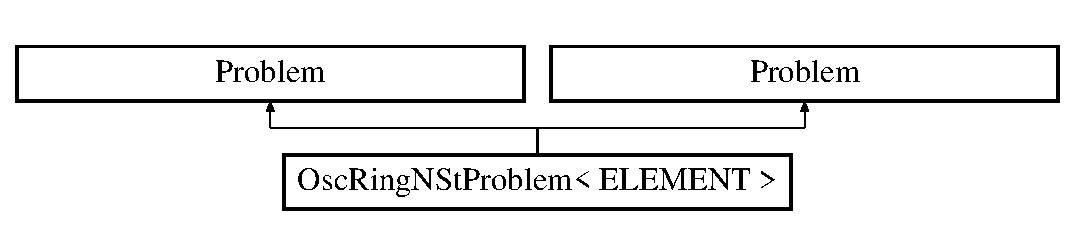
\includegraphics[height=2.000000cm]{classOscRingNStProblem}
\end{center}
\end{figure}
\subsection*{Public Member Functions}
\begin{DoxyCompactItemize}
\item 
\hyperlink{classOscRingNStProblem_acd5f633c43eb4cfb43c45361ecf85e6b}{Osc\+Ring\+N\+St\+Problem} (const double \&dt, Finite\+Element\+::\+Unsteady\+Exact\+Solution\+Fct\+Pt I\+C\+\_\+fct\+\_\+pt)
\begin{DoxyCompactList}\small\item\em Constructor\+: Pass timestep and function pointer to the solution that provides the initial conditions for the fluid. \end{DoxyCompactList}\item 
\hyperlink{classOscRingNStProblem_a96e43adf75d4e33270218ceb3397443c}{$\sim$\+Osc\+Ring\+N\+St\+Problem} ()
\begin{DoxyCompactList}\small\item\em Destructor (empty) \end{DoxyCompactList}\item 
Geom\+Object $\ast$ \hyperlink{classOscRingNStProblem_a8ef3175a1869d5d2f788c68e1c090538}{wall\+\_\+pt} ()
\begin{DoxyCompactList}\small\item\em Get pointer to wall as geometric object. \end{DoxyCompactList}\item 
void \hyperlink{classOscRingNStProblem_a6e4be6a46ab263941b76ab4e6706f63a}{actions\+\_\+after\+\_\+newton\+\_\+solve} ()
\begin{DoxyCompactList}\small\item\em Update after solve (empty) \end{DoxyCompactList}\item 
void \hyperlink{classOscRingNStProblem_a7d8ff9543c042752b649ed326d6c5915}{actions\+\_\+before\+\_\+newton\+\_\+solve} ()
\begin{DoxyCompactList}\small\item\em Update the problem specs before solve (empty) \end{DoxyCompactList}\item 
void \hyperlink{classOscRingNStProblem_a98d4c847cd9d53ab3569b8418ecb0c6b}{actions\+\_\+before\+\_\+newton\+\_\+convergence\+\_\+check} ()
\begin{DoxyCompactList}\small\item\em Update the problem specs before checking Newton convergence\+: Update the fluid mesh and re-\/set velocity boundary conditions -- no slip velocity on the wall means that the velocity on the wall is enslaved. \end{DoxyCompactList}\item 
void \hyperlink{classOscRingNStProblem_a2dd1cb9b211f2cbd2ea9aea625685bcb}{actions\+\_\+after\+\_\+adapt} ()
\begin{DoxyCompactList}\small\item\em Update the problem specs after adaptation\+: Set auxiliary update function that applies no slip on all boundary nodes and choose fluid pressure dof that drives the wall deformation. \end{DoxyCompactList}\item 
void \hyperlink{classOscRingNStProblem_a00e957fb6a313a9c1de784d0fa3a7a36}{unsteady\+\_\+run} (const unsigned \&ntsteps, const bool \&restarted, Doc\+Info \&doc\+\_\+info)
\begin{DoxyCompactList}\small\item\em Run the time integration for ntsteps steps. \end{DoxyCompactList}\item 
void \hyperlink{classOscRingNStProblem_ab1f2083699d00da4b7f6116e10792e86}{set\+\_\+initial\+\_\+condition} ()
\begin{DoxyCompactList}\small\item\em Set initial condition (incl previous timesteps) according to specified function. \end{DoxyCompactList}\item 
void \hyperlink{classOscRingNStProblem_a7de5df21c2179db1c97cc83332dcc82c}{doc\+\_\+solution} (Doc\+Info \&doc\+\_\+info)
\begin{DoxyCompactList}\small\item\em Doc the solution. \end{DoxyCompactList}\item 
Algebraic\+Refineable\+Quarter\+Circle\+Sector\+Mesh$<$ E\+L\+E\+M\+E\+NT $>$ $\ast$ \hyperlink{classOscRingNStProblem_ae9749337fca6dff52ac6e530c6339faa}{fluid\+\_\+mesh\+\_\+pt} ()
\begin{DoxyCompactList}\small\item\em Access function for the fluid mesh. \end{DoxyCompactList}\item 
void \hyperlink{classOscRingNStProblem_af32f94658174188b1f029446161755b2}{dump\+\_\+it} (ofstream \&dump\+\_\+file, Doc\+Info doc\+\_\+info)
\begin{DoxyCompactList}\small\item\em Dump problem data. \end{DoxyCompactList}\item 
void \hyperlink{classOscRingNStProblem_a0cf01737b8d53213d644413e84251d0f}{restart} (ifstream \&restart\+\_\+file)
\begin{DoxyCompactList}\small\item\em Read problem data. \end{DoxyCompactList}\item 
\hyperlink{classOscRingNStProblem_acd5f633c43eb4cfb43c45361ecf85e6b}{Osc\+Ring\+N\+St\+Problem} (const double \&dt, Finite\+Element\+::\+Unsteady\+Exact\+Solution\+Fct\+Pt I\+C\+\_\+fct\+\_\+pt)
\begin{DoxyCompactList}\small\item\em Constructor\+: Pass timestep and function pointer to the solution that provides the initial conditions for the fluid. \end{DoxyCompactList}\item 
\hyperlink{classOscRingNStProblem_a96e43adf75d4e33270218ceb3397443c}{$\sim$\+Osc\+Ring\+N\+St\+Problem} ()
\begin{DoxyCompactList}\small\item\em Destructor (empty) \end{DoxyCompactList}\item 
Geom\+Object $\ast$ \hyperlink{classOscRingNStProblem_a8ef3175a1869d5d2f788c68e1c090538}{wall\+\_\+pt} ()
\begin{DoxyCompactList}\small\item\em Get pointer to wall as geometric object. \end{DoxyCompactList}\item 
void \hyperlink{classOscRingNStProblem_a6e4be6a46ab263941b76ab4e6706f63a}{actions\+\_\+after\+\_\+newton\+\_\+solve} ()
\begin{DoxyCompactList}\small\item\em Update after solve (empty) \end{DoxyCompactList}\item 
void \hyperlink{classOscRingNStProblem_a7d8ff9543c042752b649ed326d6c5915}{actions\+\_\+before\+\_\+newton\+\_\+solve} ()
\begin{DoxyCompactList}\small\item\em Update the problem specs before solve (empty) \end{DoxyCompactList}\item 
void \hyperlink{classOscRingNStProblem_a98d4c847cd9d53ab3569b8418ecb0c6b}{actions\+\_\+before\+\_\+newton\+\_\+convergence\+\_\+check} ()
\begin{DoxyCompactList}\small\item\em Update the problem specs before checking Newton convergence\+: Update the fluid mesh and re-\/set velocity boundary conditions -- no slip velocity on the wall means that the velocity on the wall is enslaved. \end{DoxyCompactList}\item 
void \hyperlink{classOscRingNStProblem_a2dd1cb9b211f2cbd2ea9aea625685bcb}{actions\+\_\+after\+\_\+adapt} ()
\begin{DoxyCompactList}\small\item\em Update the problem specs after adaptation\+: Set auxiliary update function that applies no slip on all boundary nodes and choose fluid pressure dof that drives the wall deformation. \end{DoxyCompactList}\item 
void \hyperlink{classOscRingNStProblem_a00e957fb6a313a9c1de784d0fa3a7a36}{unsteady\+\_\+run} (const unsigned \&ntsteps, const bool \&restarted, Doc\+Info \&doc\+\_\+info)
\begin{DoxyCompactList}\small\item\em Run the time integration for ntsteps steps. \end{DoxyCompactList}\item 
void \hyperlink{classOscRingNStProblem_ab1f2083699d00da4b7f6116e10792e86}{set\+\_\+initial\+\_\+condition} ()
\begin{DoxyCompactList}\small\item\em Set initial condition (incl previous timesteps) according to specified function. \end{DoxyCompactList}\item 
void \hyperlink{classOscRingNStProblem_a7de5df21c2179db1c97cc83332dcc82c}{doc\+\_\+solution} (Doc\+Info \&doc\+\_\+info)
\begin{DoxyCompactList}\small\item\em Doc the solution. \end{DoxyCompactList}\item 
Macro\+Element\+Node\+Update\+Refineable\+Quarter\+Circle\+Sector\+Mesh$<$ E\+L\+E\+M\+E\+NT $>$ $\ast$ \hyperlink{classOscRingNStProblem_a9c0a167a315009ff298b4c43967aba9a}{fluid\+\_\+mesh\+\_\+pt} ()
\begin{DoxyCompactList}\small\item\em Access function for the fluid mesh. \end{DoxyCompactList}\item 
void \hyperlink{classOscRingNStProblem_af32f94658174188b1f029446161755b2}{dump\+\_\+it} (ofstream \&dump\+\_\+file, Doc\+Info doc\+\_\+info)
\begin{DoxyCompactList}\small\item\em Dump problem data. \end{DoxyCompactList}\item 
void \hyperlink{classOscRingNStProblem_a0cf01737b8d53213d644413e84251d0f}{restart} (ifstream \&restart\+\_\+file)
\begin{DoxyCompactList}\small\item\em Read problem data. \end{DoxyCompactList}\end{DoxyCompactItemize}
\subsection*{Private Member Functions}
\begin{DoxyCompactItemize}
\item 
void \hyperlink{classOscRingNStProblem_a96e12e5bb761d765ebe9065b9990112f}{write\+\_\+trace\+\_\+file\+\_\+header} ()
\begin{DoxyCompactList}\small\item\em Write header for trace file. \end{DoxyCompactList}\item 
void \hyperlink{classOscRingNStProblem_a96e12e5bb761d765ebe9065b9990112f}{write\+\_\+trace\+\_\+file\+\_\+header} ()
\begin{DoxyCompactList}\small\item\em Write header for trace file. \end{DoxyCompactList}\end{DoxyCompactItemize}
\subsection*{Private Attributes}
\begin{DoxyCompactItemize}
\item 
Finite\+Element\+::\+Unsteady\+Exact\+Solution\+Fct\+Pt \hyperlink{classOscRingNStProblem_ad9b2810092588c7708660c5325c73256}{I\+C\+\_\+\+Fct\+\_\+pt}
\begin{DoxyCompactList}\small\item\em Function pointer to set the intial condition. \end{DoxyCompactList}\item 
Geom\+Object $\ast$ \hyperlink{classOscRingNStProblem_a1349ecb860cacb34792fde6807d92905}{Wall\+\_\+pt}
\begin{DoxyCompactList}\small\item\em Pointer to wall. \end{DoxyCompactList}\item 
Algebraic\+Refineable\+Quarter\+Circle\+Sector\+Mesh$<$ E\+L\+E\+M\+E\+NT $>$ $\ast$ \hyperlink{classOscRingNStProblem_af9ccaa9a5c41ffadda773d704793c76e}{Fluid\+\_\+mesh\+\_\+pt}
\begin{DoxyCompactList}\small\item\em Pointer to fluid mesh. \end{DoxyCompactList}\item 
Mesh $\ast$ \hyperlink{classOscRingNStProblem_aafee49228dbbee7178448da624b96c3f}{Wall\+\_\+mesh\+\_\+pt}
\begin{DoxyCompactList}\small\item\em Pointer to wall mesh (contains only a single Generalised\+Element) \end{DoxyCompactList}\item 
ofstream \hyperlink{classOscRingNStProblem_a37c1af48245859045bed1c3fc36be3da}{Trace\+\_\+file}
\begin{DoxyCompactList}\small\item\em Trace file. \end{DoxyCompactList}\item 
Node $\ast$ \hyperlink{classOscRingNStProblem_aed51269a285ffdc064739d6d363b1179}{Veloc\+\_\+trace\+\_\+node\+\_\+pt}
\begin{DoxyCompactList}\small\item\em Pointer to node on coarsest mesh on which velocity is traced. \end{DoxyCompactList}\item 
Node $\ast$ \hyperlink{classOscRingNStProblem_a6688cac5da1f4092a9cd343ad5fdfd53}{Sarah\+\_\+veloc\+\_\+trace\+\_\+node\+\_\+pt}
\begin{DoxyCompactList}\small\item\em Pointer to node in symmetry plane on coarsest mesh at which velocity is traced. \end{DoxyCompactList}\item 
Macro\+Element\+Node\+Update\+Refineable\+Quarter\+Circle\+Sector\+Mesh$<$ E\+L\+E\+M\+E\+NT $>$ $\ast$ \hyperlink{classOscRingNStProblem_a7747a4f4f3bcc507376ca09649fcf6fd}{Fluid\+\_\+mesh\+\_\+pt}
\begin{DoxyCompactList}\small\item\em Pointer to fluid mesh. \end{DoxyCompactList}\end{DoxyCompactItemize}


\subsection{Detailed Description}
\subsubsection*{template$<$class E\+L\+E\+M\+E\+NT$>$\newline
class Osc\+Ring\+N\+St\+Problem$<$ E\+L\+E\+M\+E\+N\+T $>$}

Driver for oscillating ring problem\+: Wall performs oscillations that resemble eigenmodes of freely oscillating ring and drives viscous fluid flow. Mean radius of wall is adjustable and responds to a pressure value in the fluid to allow for mass conservation. 

Definition at line 89 of file osc\+\_\+ring\+\_\+alg.\+cc.



\subsection{Constructor \& Destructor Documentation}
\mbox{\Hypertarget{classOscRingNStProblem_acd5f633c43eb4cfb43c45361ecf85e6b}\label{classOscRingNStProblem_acd5f633c43eb4cfb43c45361ecf85e6b}} 
\index{Osc\+Ring\+N\+St\+Problem@{Osc\+Ring\+N\+St\+Problem}!Osc\+Ring\+N\+St\+Problem@{Osc\+Ring\+N\+St\+Problem}}
\index{Osc\+Ring\+N\+St\+Problem@{Osc\+Ring\+N\+St\+Problem}!Osc\+Ring\+N\+St\+Problem@{Osc\+Ring\+N\+St\+Problem}}
\subsubsection{\texorpdfstring{Osc\+Ring\+N\+St\+Problem()}{OscRingNStProblem()}\hspace{0.1cm}{\footnotesize\ttfamily [1/2]}}
{\footnotesize\ttfamily template$<$class E\+L\+E\+M\+E\+NT $>$ \\
\hyperlink{classOscRingNStProblem}{Osc\+Ring\+N\+St\+Problem}$<$ E\+L\+E\+M\+E\+NT $>$\+::\hyperlink{classOscRingNStProblem}{Osc\+Ring\+N\+St\+Problem} (\begin{DoxyParamCaption}\item[{const double \&}]{dt,  }\item[{Finite\+Element\+::\+Unsteady\+Exact\+Solution\+Fct\+Pt}]{I\+C\+\_\+fct\+\_\+pt }\end{DoxyParamCaption})}



Constructor\+: Pass timestep and function pointer to the solution that provides the initial conditions for the fluid. 

Constructor\+: Pass (constant) timestep and function pointer to the solution that provides the initial conditions for the fluid. 

Definition at line 213 of file osc\+\_\+ring\+\_\+alg.\+cc.



References oomph\+::\+Sarah\+B\+L\+::A, oomph\+::\+Sarah\+B\+L\+::alpha, oomph\+::\+Sarah\+B\+L\+::epsilon, Osc\+Ring\+N\+St\+Problem$<$ E\+L\+E\+M\+E\+N\+T $>$\+::fluid\+\_\+mesh\+\_\+pt(), Osc\+Ring\+N\+St\+Problem$<$ E\+L\+E\+M\+E\+N\+T $>$\+::\+Fluid\+\_\+mesh\+\_\+pt, oomph\+::\+Sarah\+B\+L\+::N, oomph\+::\+Sarah\+B\+L\+::\+Omega, Global\+\_\+\+Physical\+\_\+\+Variables\+::\+Re, Global\+\_\+\+Physical\+\_\+\+Variables\+::\+Re\+St, Osc\+Ring\+N\+St\+Problem$<$ E\+L\+E\+M\+E\+N\+T $>$\+::\+Sarah\+\_\+veloc\+\_\+trace\+\_\+node\+\_\+pt, Osc\+Ring\+N\+St\+Problem$<$ E\+L\+E\+M\+E\+N\+T $>$\+::\+Veloc\+\_\+trace\+\_\+node\+\_\+pt, Osc\+Ring\+N\+St\+Problem$<$ E\+L\+E\+M\+E\+N\+T $>$\+::\+Wall\+\_\+mesh\+\_\+pt, and Osc\+Ring\+N\+St\+Problem$<$ E\+L\+E\+M\+E\+N\+T $>$\+::\+Wall\+\_\+pt.

\mbox{\Hypertarget{classOscRingNStProblem_a96e43adf75d4e33270218ceb3397443c}\label{classOscRingNStProblem_a96e43adf75d4e33270218ceb3397443c}} 
\index{Osc\+Ring\+N\+St\+Problem@{Osc\+Ring\+N\+St\+Problem}!````~Osc\+Ring\+N\+St\+Problem@{$\sim$\+Osc\+Ring\+N\+St\+Problem}}
\index{````~Osc\+Ring\+N\+St\+Problem@{$\sim$\+Osc\+Ring\+N\+St\+Problem}!Osc\+Ring\+N\+St\+Problem@{Osc\+Ring\+N\+St\+Problem}}
\subsubsection{\texorpdfstring{$\sim$\+Osc\+Ring\+N\+St\+Problem()}{~OscRingNStProblem()}\hspace{0.1cm}{\footnotesize\ttfamily [1/2]}}
{\footnotesize\ttfamily template$<$class E\+L\+E\+M\+E\+NT$>$ \\
\hyperlink{classOscRingNStProblem}{Osc\+Ring\+N\+St\+Problem}$<$ E\+L\+E\+M\+E\+NT $>$\+::$\sim$\hyperlink{classOscRingNStProblem}{Osc\+Ring\+N\+St\+Problem} (\begin{DoxyParamCaption}{ }\end{DoxyParamCaption})\hspace{0.3cm}{\ttfamily [inline]}}



Destructor (empty) 



Definition at line 100 of file osc\+\_\+ring\+\_\+alg.\+cc.

\mbox{\Hypertarget{classOscRingNStProblem_acd5f633c43eb4cfb43c45361ecf85e6b}\label{classOscRingNStProblem_acd5f633c43eb4cfb43c45361ecf85e6b}} 
\index{Osc\+Ring\+N\+St\+Problem@{Osc\+Ring\+N\+St\+Problem}!Osc\+Ring\+N\+St\+Problem@{Osc\+Ring\+N\+St\+Problem}}
\index{Osc\+Ring\+N\+St\+Problem@{Osc\+Ring\+N\+St\+Problem}!Osc\+Ring\+N\+St\+Problem@{Osc\+Ring\+N\+St\+Problem}}
\subsubsection{\texorpdfstring{Osc\+Ring\+N\+St\+Problem()}{OscRingNStProblem()}\hspace{0.1cm}{\footnotesize\ttfamily [2/2]}}
{\footnotesize\ttfamily template$<$class E\+L\+E\+M\+E\+NT$>$ \\
\hyperlink{classOscRingNStProblem}{Osc\+Ring\+N\+St\+Problem}$<$ E\+L\+E\+M\+E\+NT $>$\+::\hyperlink{classOscRingNStProblem}{Osc\+Ring\+N\+St\+Problem} (\begin{DoxyParamCaption}\item[{const double \&}]{dt,  }\item[{Finite\+Element\+::\+Unsteady\+Exact\+Solution\+Fct\+Pt}]{I\+C\+\_\+fct\+\_\+pt }\end{DoxyParamCaption})}



Constructor\+: Pass timestep and function pointer to the solution that provides the initial conditions for the fluid. 

\mbox{\Hypertarget{classOscRingNStProblem_a96e43adf75d4e33270218ceb3397443c}\label{classOscRingNStProblem_a96e43adf75d4e33270218ceb3397443c}} 
\index{Osc\+Ring\+N\+St\+Problem@{Osc\+Ring\+N\+St\+Problem}!````~Osc\+Ring\+N\+St\+Problem@{$\sim$\+Osc\+Ring\+N\+St\+Problem}}
\index{````~Osc\+Ring\+N\+St\+Problem@{$\sim$\+Osc\+Ring\+N\+St\+Problem}!Osc\+Ring\+N\+St\+Problem@{Osc\+Ring\+N\+St\+Problem}}
\subsubsection{\texorpdfstring{$\sim$\+Osc\+Ring\+N\+St\+Problem()}{~OscRingNStProblem()}\hspace{0.1cm}{\footnotesize\ttfamily [2/2]}}
{\footnotesize\ttfamily template$<$class E\+L\+E\+M\+E\+NT$>$ \\
\hyperlink{classOscRingNStProblem}{Osc\+Ring\+N\+St\+Problem}$<$ E\+L\+E\+M\+E\+NT $>$\+::$\sim$\hyperlink{classOscRingNStProblem}{Osc\+Ring\+N\+St\+Problem} (\begin{DoxyParamCaption}{ }\end{DoxyParamCaption})\hspace{0.3cm}{\ttfamily [inline]}}



Destructor (empty) 



Definition at line 99 of file osc\+\_\+ring\+\_\+macro.\+cc.



\subsection{Member Function Documentation}
\mbox{\Hypertarget{classOscRingNStProblem_a2dd1cb9b211f2cbd2ea9aea625685bcb}\label{classOscRingNStProblem_a2dd1cb9b211f2cbd2ea9aea625685bcb}} 
\index{Osc\+Ring\+N\+St\+Problem@{Osc\+Ring\+N\+St\+Problem}!actions\+\_\+after\+\_\+adapt@{actions\+\_\+after\+\_\+adapt}}
\index{actions\+\_\+after\+\_\+adapt@{actions\+\_\+after\+\_\+adapt}!Osc\+Ring\+N\+St\+Problem@{Osc\+Ring\+N\+St\+Problem}}
\subsubsection{\texorpdfstring{actions\+\_\+after\+\_\+adapt()}{actions\_after\_adapt()}\hspace{0.1cm}{\footnotesize\ttfamily [1/2]}}
{\footnotesize\ttfamily template$<$class E\+L\+E\+M\+E\+NT$>$ \\
void \hyperlink{classOscRingNStProblem}{Osc\+Ring\+N\+St\+Problem}$<$ E\+L\+E\+M\+E\+NT $>$\+::actions\+\_\+after\+\_\+adapt (\begin{DoxyParamCaption}{ }\end{DoxyParamCaption})\hspace{0.3cm}{\ttfamily [inline]}}



Update the problem specs after adaptation\+: Set auxiliary update function that applies no slip on all boundary nodes and choose fluid pressure dof that drives the wall deformation. 



Definition at line 129 of file osc\+\_\+ring\+\_\+macro.\+cc.

\mbox{\Hypertarget{classOscRingNStProblem_a2dd1cb9b211f2cbd2ea9aea625685bcb}\label{classOscRingNStProblem_a2dd1cb9b211f2cbd2ea9aea625685bcb}} 
\index{Osc\+Ring\+N\+St\+Problem@{Osc\+Ring\+N\+St\+Problem}!actions\+\_\+after\+\_\+adapt@{actions\+\_\+after\+\_\+adapt}}
\index{actions\+\_\+after\+\_\+adapt@{actions\+\_\+after\+\_\+adapt}!Osc\+Ring\+N\+St\+Problem@{Osc\+Ring\+N\+St\+Problem}}
\subsubsection{\texorpdfstring{actions\+\_\+after\+\_\+adapt()}{actions\_after\_adapt()}\hspace{0.1cm}{\footnotesize\ttfamily [2/2]}}
{\footnotesize\ttfamily template$<$class E\+L\+E\+M\+E\+NT$>$ \\
void \hyperlink{classOscRingNStProblem}{Osc\+Ring\+N\+St\+Problem}$<$ E\+L\+E\+M\+E\+NT $>$\+::actions\+\_\+after\+\_\+adapt (\begin{DoxyParamCaption}{ }\end{DoxyParamCaption})\hspace{0.3cm}{\ttfamily [inline]}}



Update the problem specs after adaptation\+: Set auxiliary update function that applies no slip on all boundary nodes and choose fluid pressure dof that drives the wall deformation. 



Definition at line 130 of file osc\+\_\+ring\+\_\+alg.\+cc.

\mbox{\Hypertarget{classOscRingNStProblem_a6e4be6a46ab263941b76ab4e6706f63a}\label{classOscRingNStProblem_a6e4be6a46ab263941b76ab4e6706f63a}} 
\index{Osc\+Ring\+N\+St\+Problem@{Osc\+Ring\+N\+St\+Problem}!actions\+\_\+after\+\_\+newton\+\_\+solve@{actions\+\_\+after\+\_\+newton\+\_\+solve}}
\index{actions\+\_\+after\+\_\+newton\+\_\+solve@{actions\+\_\+after\+\_\+newton\+\_\+solve}!Osc\+Ring\+N\+St\+Problem@{Osc\+Ring\+N\+St\+Problem}}
\subsubsection{\texorpdfstring{actions\+\_\+after\+\_\+newton\+\_\+solve()}{actions\_after\_newton\_solve()}\hspace{0.1cm}{\footnotesize\ttfamily [1/2]}}
{\footnotesize\ttfamily template$<$class E\+L\+E\+M\+E\+NT$>$ \\
void \hyperlink{classOscRingNStProblem}{Osc\+Ring\+N\+St\+Problem}$<$ E\+L\+E\+M\+E\+NT $>$\+::actions\+\_\+after\+\_\+newton\+\_\+solve (\begin{DoxyParamCaption}{ }\end{DoxyParamCaption})\hspace{0.3cm}{\ttfamily [inline]}}



Update after solve (empty) 



Definition at line 108 of file osc\+\_\+ring\+\_\+macro.\+cc.

\mbox{\Hypertarget{classOscRingNStProblem_a6e4be6a46ab263941b76ab4e6706f63a}\label{classOscRingNStProblem_a6e4be6a46ab263941b76ab4e6706f63a}} 
\index{Osc\+Ring\+N\+St\+Problem@{Osc\+Ring\+N\+St\+Problem}!actions\+\_\+after\+\_\+newton\+\_\+solve@{actions\+\_\+after\+\_\+newton\+\_\+solve}}
\index{actions\+\_\+after\+\_\+newton\+\_\+solve@{actions\+\_\+after\+\_\+newton\+\_\+solve}!Osc\+Ring\+N\+St\+Problem@{Osc\+Ring\+N\+St\+Problem}}
\subsubsection{\texorpdfstring{actions\+\_\+after\+\_\+newton\+\_\+solve()}{actions\_after\_newton\_solve()}\hspace{0.1cm}{\footnotesize\ttfamily [2/2]}}
{\footnotesize\ttfamily template$<$class E\+L\+E\+M\+E\+NT$>$ \\
void \hyperlink{classOscRingNStProblem}{Osc\+Ring\+N\+St\+Problem}$<$ E\+L\+E\+M\+E\+NT $>$\+::actions\+\_\+after\+\_\+newton\+\_\+solve (\begin{DoxyParamCaption}{ }\end{DoxyParamCaption})\hspace{0.3cm}{\ttfamily [inline]}}



Update after solve (empty) 



Definition at line 109 of file osc\+\_\+ring\+\_\+alg.\+cc.

\mbox{\Hypertarget{classOscRingNStProblem_a98d4c847cd9d53ab3569b8418ecb0c6b}\label{classOscRingNStProblem_a98d4c847cd9d53ab3569b8418ecb0c6b}} 
\index{Osc\+Ring\+N\+St\+Problem@{Osc\+Ring\+N\+St\+Problem}!actions\+\_\+before\+\_\+newton\+\_\+convergence\+\_\+check@{actions\+\_\+before\+\_\+newton\+\_\+convergence\+\_\+check}}
\index{actions\+\_\+before\+\_\+newton\+\_\+convergence\+\_\+check@{actions\+\_\+before\+\_\+newton\+\_\+convergence\+\_\+check}!Osc\+Ring\+N\+St\+Problem@{Osc\+Ring\+N\+St\+Problem}}
\subsubsection{\texorpdfstring{actions\+\_\+before\+\_\+newton\+\_\+convergence\+\_\+check()}{actions\_before\_newton\_convergence\_check()}\hspace{0.1cm}{\footnotesize\ttfamily [1/2]}}
{\footnotesize\ttfamily template$<$class E\+L\+E\+M\+E\+NT$>$ \\
void \hyperlink{classOscRingNStProblem}{Osc\+Ring\+N\+St\+Problem}$<$ E\+L\+E\+M\+E\+NT $>$\+::actions\+\_\+before\+\_\+newton\+\_\+convergence\+\_\+check (\begin{DoxyParamCaption}{ }\end{DoxyParamCaption})\hspace{0.3cm}{\ttfamily [inline]}}



Update the problem specs before checking Newton convergence\+: Update the fluid mesh and re-\/set velocity boundary conditions -- no slip velocity on the wall means that the velocity on the wall is enslaved. 



Definition at line 117 of file osc\+\_\+ring\+\_\+macro.\+cc.

\mbox{\Hypertarget{classOscRingNStProblem_a98d4c847cd9d53ab3569b8418ecb0c6b}\label{classOscRingNStProblem_a98d4c847cd9d53ab3569b8418ecb0c6b}} 
\index{Osc\+Ring\+N\+St\+Problem@{Osc\+Ring\+N\+St\+Problem}!actions\+\_\+before\+\_\+newton\+\_\+convergence\+\_\+check@{actions\+\_\+before\+\_\+newton\+\_\+convergence\+\_\+check}}
\index{actions\+\_\+before\+\_\+newton\+\_\+convergence\+\_\+check@{actions\+\_\+before\+\_\+newton\+\_\+convergence\+\_\+check}!Osc\+Ring\+N\+St\+Problem@{Osc\+Ring\+N\+St\+Problem}}
\subsubsection{\texorpdfstring{actions\+\_\+before\+\_\+newton\+\_\+convergence\+\_\+check()}{actions\_before\_newton\_convergence\_check()}\hspace{0.1cm}{\footnotesize\ttfamily [2/2]}}
{\footnotesize\ttfamily template$<$class E\+L\+E\+M\+E\+NT$>$ \\
void \hyperlink{classOscRingNStProblem}{Osc\+Ring\+N\+St\+Problem}$<$ E\+L\+E\+M\+E\+NT $>$\+::actions\+\_\+before\+\_\+newton\+\_\+convergence\+\_\+check (\begin{DoxyParamCaption}{ }\end{DoxyParamCaption})\hspace{0.3cm}{\ttfamily [inline]}}



Update the problem specs before checking Newton convergence\+: Update the fluid mesh and re-\/set velocity boundary conditions -- no slip velocity on the wall means that the velocity on the wall is enslaved. 



Definition at line 118 of file osc\+\_\+ring\+\_\+alg.\+cc.

\mbox{\Hypertarget{classOscRingNStProblem_a7d8ff9543c042752b649ed326d6c5915}\label{classOscRingNStProblem_a7d8ff9543c042752b649ed326d6c5915}} 
\index{Osc\+Ring\+N\+St\+Problem@{Osc\+Ring\+N\+St\+Problem}!actions\+\_\+before\+\_\+newton\+\_\+solve@{actions\+\_\+before\+\_\+newton\+\_\+solve}}
\index{actions\+\_\+before\+\_\+newton\+\_\+solve@{actions\+\_\+before\+\_\+newton\+\_\+solve}!Osc\+Ring\+N\+St\+Problem@{Osc\+Ring\+N\+St\+Problem}}
\subsubsection{\texorpdfstring{actions\+\_\+before\+\_\+newton\+\_\+solve()}{actions\_before\_newton\_solve()}\hspace{0.1cm}{\footnotesize\ttfamily [1/2]}}
{\footnotesize\ttfamily template$<$class E\+L\+E\+M\+E\+NT$>$ \\
void \hyperlink{classOscRingNStProblem}{Osc\+Ring\+N\+St\+Problem}$<$ E\+L\+E\+M\+E\+NT $>$\+::actions\+\_\+before\+\_\+newton\+\_\+solve (\begin{DoxyParamCaption}{ }\end{DoxyParamCaption})\hspace{0.3cm}{\ttfamily [inline]}}



Update the problem specs before solve (empty) 



Definition at line 111 of file osc\+\_\+ring\+\_\+macro.\+cc.

\mbox{\Hypertarget{classOscRingNStProblem_a7d8ff9543c042752b649ed326d6c5915}\label{classOscRingNStProblem_a7d8ff9543c042752b649ed326d6c5915}} 
\index{Osc\+Ring\+N\+St\+Problem@{Osc\+Ring\+N\+St\+Problem}!actions\+\_\+before\+\_\+newton\+\_\+solve@{actions\+\_\+before\+\_\+newton\+\_\+solve}}
\index{actions\+\_\+before\+\_\+newton\+\_\+solve@{actions\+\_\+before\+\_\+newton\+\_\+solve}!Osc\+Ring\+N\+St\+Problem@{Osc\+Ring\+N\+St\+Problem}}
\subsubsection{\texorpdfstring{actions\+\_\+before\+\_\+newton\+\_\+solve()}{actions\_before\_newton\_solve()}\hspace{0.1cm}{\footnotesize\ttfamily [2/2]}}
{\footnotesize\ttfamily template$<$class E\+L\+E\+M\+E\+NT$>$ \\
void \hyperlink{classOscRingNStProblem}{Osc\+Ring\+N\+St\+Problem}$<$ E\+L\+E\+M\+E\+NT $>$\+::actions\+\_\+before\+\_\+newton\+\_\+solve (\begin{DoxyParamCaption}{ }\end{DoxyParamCaption})\hspace{0.3cm}{\ttfamily [inline]}}



Update the problem specs before solve (empty) 



Definition at line 112 of file osc\+\_\+ring\+\_\+alg.\+cc.

\mbox{\Hypertarget{classOscRingNStProblem_a7de5df21c2179db1c97cc83332dcc82c}\label{classOscRingNStProblem_a7de5df21c2179db1c97cc83332dcc82c}} 
\index{Osc\+Ring\+N\+St\+Problem@{Osc\+Ring\+N\+St\+Problem}!doc\+\_\+solution@{doc\+\_\+solution}}
\index{doc\+\_\+solution@{doc\+\_\+solution}!Osc\+Ring\+N\+St\+Problem@{Osc\+Ring\+N\+St\+Problem}}
\subsubsection{\texorpdfstring{doc\+\_\+solution()}{doc\_solution()}\hspace{0.1cm}{\footnotesize\ttfamily [1/2]}}
{\footnotesize\ttfamily template$<$class E\+L\+E\+M\+E\+NT$>$ \\
void \hyperlink{classOscRingNStProblem}{Osc\+Ring\+N\+St\+Problem}$<$ E\+L\+E\+M\+E\+NT $>$\+::doc\+\_\+solution (\begin{DoxyParamCaption}\item[{Doc\+Info \&}]{doc\+\_\+info }\end{DoxyParamCaption})}



Doc the solution. 

\mbox{\Hypertarget{classOscRingNStProblem_a7de5df21c2179db1c97cc83332dcc82c}\label{classOscRingNStProblem_a7de5df21c2179db1c97cc83332dcc82c}} 
\index{Osc\+Ring\+N\+St\+Problem@{Osc\+Ring\+N\+St\+Problem}!doc\+\_\+solution@{doc\+\_\+solution}}
\index{doc\+\_\+solution@{doc\+\_\+solution}!Osc\+Ring\+N\+St\+Problem@{Osc\+Ring\+N\+St\+Problem}}
\subsubsection{\texorpdfstring{doc\+\_\+solution()}{doc\_solution()}\hspace{0.1cm}{\footnotesize\ttfamily [2/2]}}
{\footnotesize\ttfamily template$<$class E\+L\+E\+M\+E\+NT $>$ \\
void \hyperlink{classOscRingNStProblem}{Osc\+Ring\+N\+St\+Problem}$<$ E\+L\+E\+M\+E\+NT $>$\+::doc\+\_\+solution (\begin{DoxyParamCaption}\item[{Doc\+Info \&}]{doc\+\_\+info }\end{DoxyParamCaption})}



Doc the solution. 

Doc the solution 

Definition at line 490 of file osc\+\_\+ring\+\_\+alg.\+cc.



References Osc\+Ring\+N\+St\+Problem$<$ E\+L\+E\+M\+E\+N\+T $>$\+::dump\+\_\+it(), oomph\+::\+Sarah\+B\+L\+::exact\+\_\+soln(), Osc\+Ring\+N\+St\+Problem$<$ E\+L\+E\+M\+E\+N\+T $>$\+::fluid\+\_\+mesh\+\_\+pt(), oomph\+::\+Sarah\+B\+L\+::full\+\_\+exact\+\_\+soln(), oomph\+::\+Sarah\+B\+L\+::\+Kin\+\_\+energy\+\_\+sarah(), Osc\+Ring\+N\+St\+Problem$<$ E\+L\+E\+M\+E\+N\+T $>$\+::\+Sarah\+\_\+veloc\+\_\+trace\+\_\+node\+\_\+pt, oomph\+::\+Sarah\+B\+L\+::\+Total\+\_\+\+Diss\+\_\+sarah(), Osc\+Ring\+N\+St\+Problem$<$ E\+L\+E\+M\+E\+N\+T $>$\+::\+Trace\+\_\+file, Osc\+Ring\+N\+St\+Problem$<$ E\+L\+E\+M\+E\+N\+T $>$\+::\+Veloc\+\_\+trace\+\_\+node\+\_\+pt, Osc\+Ring\+N\+St\+Problem$<$ E\+L\+E\+M\+E\+N\+T $>$\+::wall\+\_\+pt(), and Osc\+Ring\+N\+St\+Problem$<$ E\+L\+E\+M\+E\+N\+T $>$\+::\+Wall\+\_\+pt.



Referenced by Osc\+Ring\+N\+St\+Problem$<$ E\+L\+E\+M\+E\+N\+T $>$\+::unsteady\+\_\+run().

\mbox{\Hypertarget{classOscRingNStProblem_af32f94658174188b1f029446161755b2}\label{classOscRingNStProblem_af32f94658174188b1f029446161755b2}} 
\index{Osc\+Ring\+N\+St\+Problem@{Osc\+Ring\+N\+St\+Problem}!dump\+\_\+it@{dump\+\_\+it}}
\index{dump\+\_\+it@{dump\+\_\+it}!Osc\+Ring\+N\+St\+Problem@{Osc\+Ring\+N\+St\+Problem}}
\subsubsection{\texorpdfstring{dump\+\_\+it()}{dump\_it()}\hspace{0.1cm}{\footnotesize\ttfamily [1/2]}}
{\footnotesize\ttfamily template$<$class E\+L\+E\+M\+E\+NT$>$ \\
void \hyperlink{classOscRingNStProblem}{Osc\+Ring\+N\+St\+Problem}$<$ E\+L\+E\+M\+E\+NT $>$\+::dump\+\_\+it (\begin{DoxyParamCaption}\item[{ofstream \&}]{dump\+\_\+file,  }\item[{Doc\+Info}]{doc\+\_\+info }\end{DoxyParamCaption})}



Dump problem data. 

\mbox{\Hypertarget{classOscRingNStProblem_af32f94658174188b1f029446161755b2}\label{classOscRingNStProblem_af32f94658174188b1f029446161755b2}} 
\index{Osc\+Ring\+N\+St\+Problem@{Osc\+Ring\+N\+St\+Problem}!dump\+\_\+it@{dump\+\_\+it}}
\index{dump\+\_\+it@{dump\+\_\+it}!Osc\+Ring\+N\+St\+Problem@{Osc\+Ring\+N\+St\+Problem}}
\subsubsection{\texorpdfstring{dump\+\_\+it()}{dump\_it()}\hspace{0.1cm}{\footnotesize\ttfamily [2/2]}}
{\footnotesize\ttfamily template$<$class E\+L\+E\+M\+E\+NT $>$ \\
void \hyperlink{classOscRingNStProblem}{Osc\+Ring\+N\+St\+Problem}$<$ E\+L\+E\+M\+E\+NT $>$\+::dump\+\_\+it (\begin{DoxyParamCaption}\item[{ofstream \&}]{dump\+\_\+file,  }\item[{Doc\+Info}]{doc\+\_\+info }\end{DoxyParamCaption})}



Dump problem data. 

Dump the solution. 

Definition at line 691 of file osc\+\_\+ring\+\_\+alg.\+cc.



Referenced by Osc\+Ring\+N\+St\+Problem$<$ E\+L\+E\+M\+E\+N\+T $>$\+::doc\+\_\+solution().

\mbox{\Hypertarget{classOscRingNStProblem_a9c0a167a315009ff298b4c43967aba9a}\label{classOscRingNStProblem_a9c0a167a315009ff298b4c43967aba9a}} 
\index{Osc\+Ring\+N\+St\+Problem@{Osc\+Ring\+N\+St\+Problem}!fluid\+\_\+mesh\+\_\+pt@{fluid\+\_\+mesh\+\_\+pt}}
\index{fluid\+\_\+mesh\+\_\+pt@{fluid\+\_\+mesh\+\_\+pt}!Osc\+Ring\+N\+St\+Problem@{Osc\+Ring\+N\+St\+Problem}}
\subsubsection{\texorpdfstring{fluid\+\_\+mesh\+\_\+pt()}{fluid\_mesh\_pt()}\hspace{0.1cm}{\footnotesize\ttfamily [1/2]}}
{\footnotesize\ttfamily template$<$class E\+L\+E\+M\+E\+NT$>$ \\
Macro\+Element\+Node\+Update\+Refineable\+Quarter\+Circle\+Sector\+Mesh$<$E\+L\+E\+M\+E\+NT$>$$\ast$ \hyperlink{classOscRingNStProblem}{Osc\+Ring\+N\+St\+Problem}$<$ E\+L\+E\+M\+E\+NT $>$\+::fluid\+\_\+mesh\+\_\+pt (\begin{DoxyParamCaption}{ }\end{DoxyParamCaption})\hspace{0.3cm}{\ttfamily [inline]}}



Access function for the fluid mesh. 



Definition at line 166 of file osc\+\_\+ring\+\_\+macro.\+cc.

\mbox{\Hypertarget{classOscRingNStProblem_ae9749337fca6dff52ac6e530c6339faa}\label{classOscRingNStProblem_ae9749337fca6dff52ac6e530c6339faa}} 
\index{Osc\+Ring\+N\+St\+Problem@{Osc\+Ring\+N\+St\+Problem}!fluid\+\_\+mesh\+\_\+pt@{fluid\+\_\+mesh\+\_\+pt}}
\index{fluid\+\_\+mesh\+\_\+pt@{fluid\+\_\+mesh\+\_\+pt}!Osc\+Ring\+N\+St\+Problem@{Osc\+Ring\+N\+St\+Problem}}
\subsubsection{\texorpdfstring{fluid\+\_\+mesh\+\_\+pt()}{fluid\_mesh\_pt()}\hspace{0.1cm}{\footnotesize\ttfamily [2/2]}}
{\footnotesize\ttfamily template$<$class E\+L\+E\+M\+E\+NT$>$ \\
Algebraic\+Refineable\+Quarter\+Circle\+Sector\+Mesh$<$E\+L\+E\+M\+E\+NT$>$$\ast$ \hyperlink{classOscRingNStProblem}{Osc\+Ring\+N\+St\+Problem}$<$ E\+L\+E\+M\+E\+NT $>$\+::fluid\+\_\+mesh\+\_\+pt (\begin{DoxyParamCaption}{ }\end{DoxyParamCaption})\hspace{0.3cm}{\ttfamily [inline]}}



Access function for the fluid mesh. 



Definition at line 167 of file osc\+\_\+ring\+\_\+alg.\+cc.



Referenced by Osc\+Ring\+N\+St\+Problem$<$ E\+L\+E\+M\+E\+N\+T $>$\+::doc\+\_\+solution(), Osc\+Ring\+N\+St\+Problem$<$ E\+L\+E\+M\+E\+N\+T $>$\+::\+Osc\+Ring\+N\+St\+Problem(), Osc\+Ring\+N\+St\+Problem$<$ E\+L\+E\+M\+E\+N\+T $>$\+::set\+\_\+initial\+\_\+condition(), Osc\+Ring\+N\+St\+Problem$<$ E\+L\+E\+M\+E\+N\+T $>$\+::unsteady\+\_\+run(), and Osc\+Ring\+N\+St\+Problem$<$ E\+L\+E\+M\+E\+N\+T $>$\+::write\+\_\+trace\+\_\+file\+\_\+header().

\mbox{\Hypertarget{classOscRingNStProblem_a0cf01737b8d53213d644413e84251d0f}\label{classOscRingNStProblem_a0cf01737b8d53213d644413e84251d0f}} 
\index{Osc\+Ring\+N\+St\+Problem@{Osc\+Ring\+N\+St\+Problem}!restart@{restart}}
\index{restart@{restart}!Osc\+Ring\+N\+St\+Problem@{Osc\+Ring\+N\+St\+Problem}}
\subsubsection{\texorpdfstring{restart()}{restart()}\hspace{0.1cm}{\footnotesize\ttfamily [1/2]}}
{\footnotesize\ttfamily template$<$class E\+L\+E\+M\+E\+NT$>$ \\
void \hyperlink{classOscRingNStProblem}{Osc\+Ring\+N\+St\+Problem}$<$ E\+L\+E\+M\+E\+NT $>$\+::restart (\begin{DoxyParamCaption}\item[{ifstream \&}]{restart\+\_\+file }\end{DoxyParamCaption})}



Read problem data. 

\mbox{\Hypertarget{classOscRingNStProblem_a0cf01737b8d53213d644413e84251d0f}\label{classOscRingNStProblem_a0cf01737b8d53213d644413e84251d0f}} 
\index{Osc\+Ring\+N\+St\+Problem@{Osc\+Ring\+N\+St\+Problem}!restart@{restart}}
\index{restart@{restart}!Osc\+Ring\+N\+St\+Problem@{Osc\+Ring\+N\+St\+Problem}}
\subsubsection{\texorpdfstring{restart()}{restart()}\hspace{0.1cm}{\footnotesize\ttfamily [2/2]}}
{\footnotesize\ttfamily template$<$class E\+L\+E\+M\+E\+NT $>$ \\
void \hyperlink{classOscRingNStProblem}{Osc\+Ring\+N\+St\+Problem}$<$ E\+L\+E\+M\+E\+NT $>$\+::restart (\begin{DoxyParamCaption}\item[{ifstream \&}]{restart\+\_\+file }\end{DoxyParamCaption})}



Read problem data. 

Read solution from disk. 

Definition at line 708 of file osc\+\_\+ring\+\_\+alg.\+cc.



Referenced by main().

\mbox{\Hypertarget{classOscRingNStProblem_ab1f2083699d00da4b7f6116e10792e86}\label{classOscRingNStProblem_ab1f2083699d00da4b7f6116e10792e86}} 
\index{Osc\+Ring\+N\+St\+Problem@{Osc\+Ring\+N\+St\+Problem}!set\+\_\+initial\+\_\+condition@{set\+\_\+initial\+\_\+condition}}
\index{set\+\_\+initial\+\_\+condition@{set\+\_\+initial\+\_\+condition}!Osc\+Ring\+N\+St\+Problem@{Osc\+Ring\+N\+St\+Problem}}
\subsubsection{\texorpdfstring{set\+\_\+initial\+\_\+condition()}{set\_initial\_condition()}\hspace{0.1cm}{\footnotesize\ttfamily [1/2]}}
{\footnotesize\ttfamily template$<$class E\+L\+E\+M\+E\+NT$>$ \\
void \hyperlink{classOscRingNStProblem}{Osc\+Ring\+N\+St\+Problem}$<$ E\+L\+E\+M\+E\+NT $>$\+::set\+\_\+initial\+\_\+condition (\begin{DoxyParamCaption}{ }\end{DoxyParamCaption})}



Set initial condition (incl previous timesteps) according to specified function. 

\mbox{\Hypertarget{classOscRingNStProblem_ab1f2083699d00da4b7f6116e10792e86}\label{classOscRingNStProblem_ab1f2083699d00da4b7f6116e10792e86}} 
\index{Osc\+Ring\+N\+St\+Problem@{Osc\+Ring\+N\+St\+Problem}!set\+\_\+initial\+\_\+condition@{set\+\_\+initial\+\_\+condition}}
\index{set\+\_\+initial\+\_\+condition@{set\+\_\+initial\+\_\+condition}!Osc\+Ring\+N\+St\+Problem@{Osc\+Ring\+N\+St\+Problem}}
\subsubsection{\texorpdfstring{set\+\_\+initial\+\_\+condition()}{set\_initial\_condition()}\hspace{0.1cm}{\footnotesize\ttfamily [2/2]}}
{\footnotesize\ttfamily template$<$class E\+L\+E\+M\+E\+NT $>$ \\
void \hyperlink{classOscRingNStProblem}{Osc\+Ring\+N\+St\+Problem}$<$ E\+L\+E\+M\+E\+NT $>$\+::set\+\_\+initial\+\_\+condition (\begin{DoxyParamCaption}{ }\end{DoxyParamCaption})}



Set initial condition (incl previous timesteps) according to specified function. 

Set initial condition\+: Assign previous and current values of the velocity from the velocity field specified via the function pointer.

Values are assigned so that the velocities and accelerations are correct for current time. 

Definition at line 404 of file osc\+\_\+ring\+\_\+alg.\+cc.



References Osc\+Ring\+N\+St\+Problem$<$ E\+L\+E\+M\+E\+N\+T $>$\+::fluid\+\_\+mesh\+\_\+pt(), and Osc\+Ring\+N\+St\+Problem$<$ E\+L\+E\+M\+E\+N\+T $>$\+::\+Wall\+\_\+pt.



Referenced by main().

\mbox{\Hypertarget{classOscRingNStProblem_a00e957fb6a313a9c1de784d0fa3a7a36}\label{classOscRingNStProblem_a00e957fb6a313a9c1de784d0fa3a7a36}} 
\index{Osc\+Ring\+N\+St\+Problem@{Osc\+Ring\+N\+St\+Problem}!unsteady\+\_\+run@{unsteady\+\_\+run}}
\index{unsteady\+\_\+run@{unsteady\+\_\+run}!Osc\+Ring\+N\+St\+Problem@{Osc\+Ring\+N\+St\+Problem}}
\subsubsection{\texorpdfstring{unsteady\+\_\+run()}{unsteady\_run()}\hspace{0.1cm}{\footnotesize\ttfamily [1/2]}}
{\footnotesize\ttfamily template$<$class E\+L\+E\+M\+E\+NT$>$ \\
void \hyperlink{classOscRingNStProblem}{Osc\+Ring\+N\+St\+Problem}$<$ E\+L\+E\+M\+E\+NT $>$\+::unsteady\+\_\+run (\begin{DoxyParamCaption}\item[{const unsigned \&}]{ntsteps,  }\item[{const bool \&}]{restarted,  }\item[{Doc\+Info \&}]{doc\+\_\+info }\end{DoxyParamCaption})}



Run the time integration for ntsteps steps. 

\mbox{\Hypertarget{classOscRingNStProblem_a00e957fb6a313a9c1de784d0fa3a7a36}\label{classOscRingNStProblem_a00e957fb6a313a9c1de784d0fa3a7a36}} 
\index{Osc\+Ring\+N\+St\+Problem@{Osc\+Ring\+N\+St\+Problem}!unsteady\+\_\+run@{unsteady\+\_\+run}}
\index{unsteady\+\_\+run@{unsteady\+\_\+run}!Osc\+Ring\+N\+St\+Problem@{Osc\+Ring\+N\+St\+Problem}}
\subsubsection{\texorpdfstring{unsteady\+\_\+run()}{unsteady\_run()}\hspace{0.1cm}{\footnotesize\ttfamily [2/2]}}
{\footnotesize\ttfamily template$<$class E\+L\+E\+M\+E\+NT $>$ \\
void \hyperlink{classOscRingNStProblem}{Osc\+Ring\+N\+St\+Problem}$<$ E\+L\+E\+M\+E\+NT $>$\+::unsteady\+\_\+run (\begin{DoxyParamCaption}\item[{const unsigned \&}]{ntsteps,  }\item[{const bool \&}]{restarted,  }\item[{Doc\+Info \&}]{doc\+\_\+info }\end{DoxyParamCaption})}



Run the time integration for ntsteps steps. 

Driver for timestepping the problem\+: Fixed timestep but guaranteed spatial accuracy. Beautiful, innit? 

Definition at line 735 of file osc\+\_\+ring\+\_\+alg.\+cc.



References Osc\+Ring\+N\+St\+Problem$<$ E\+L\+E\+M\+E\+N\+T $>$\+::doc\+\_\+solution(), Osc\+Ring\+N\+St\+Problem$<$ E\+L\+E\+M\+E\+N\+T $>$\+::fluid\+\_\+mesh\+\_\+pt(), Osc\+Ring\+N\+St\+Problem$<$ E\+L\+E\+M\+E\+N\+T $>$\+::\+Trace\+\_\+file, and Osc\+Ring\+N\+St\+Problem$<$ E\+L\+E\+M\+E\+N\+T $>$\+::write\+\_\+trace\+\_\+file\+\_\+header().



Referenced by main().

\mbox{\Hypertarget{classOscRingNStProblem_a8ef3175a1869d5d2f788c68e1c090538}\label{classOscRingNStProblem_a8ef3175a1869d5d2f788c68e1c090538}} 
\index{Osc\+Ring\+N\+St\+Problem@{Osc\+Ring\+N\+St\+Problem}!wall\+\_\+pt@{wall\+\_\+pt}}
\index{wall\+\_\+pt@{wall\+\_\+pt}!Osc\+Ring\+N\+St\+Problem@{Osc\+Ring\+N\+St\+Problem}}
\subsubsection{\texorpdfstring{wall\+\_\+pt()}{wall\_pt()}\hspace{0.1cm}{\footnotesize\ttfamily [1/2]}}
{\footnotesize\ttfamily template$<$class E\+L\+E\+M\+E\+NT$>$ \\
Geom\+Object$\ast$ \hyperlink{classOscRingNStProblem}{Osc\+Ring\+N\+St\+Problem}$<$ E\+L\+E\+M\+E\+NT $>$\+::wall\+\_\+pt (\begin{DoxyParamCaption}{ }\end{DoxyParamCaption})\hspace{0.3cm}{\ttfamily [inline]}}



Get pointer to wall as geometric object. 



Definition at line 102 of file osc\+\_\+ring\+\_\+macro.\+cc.

\mbox{\Hypertarget{classOscRingNStProblem_a8ef3175a1869d5d2f788c68e1c090538}\label{classOscRingNStProblem_a8ef3175a1869d5d2f788c68e1c090538}} 
\index{Osc\+Ring\+N\+St\+Problem@{Osc\+Ring\+N\+St\+Problem}!wall\+\_\+pt@{wall\+\_\+pt}}
\index{wall\+\_\+pt@{wall\+\_\+pt}!Osc\+Ring\+N\+St\+Problem@{Osc\+Ring\+N\+St\+Problem}}
\subsubsection{\texorpdfstring{wall\+\_\+pt()}{wall\_pt()}\hspace{0.1cm}{\footnotesize\ttfamily [2/2]}}
{\footnotesize\ttfamily template$<$class E\+L\+E\+M\+E\+NT$>$ \\
Geom\+Object$\ast$ \hyperlink{classOscRingNStProblem}{Osc\+Ring\+N\+St\+Problem}$<$ E\+L\+E\+M\+E\+NT $>$\+::wall\+\_\+pt (\begin{DoxyParamCaption}{ }\end{DoxyParamCaption})\hspace{0.3cm}{\ttfamily [inline]}}



Get pointer to wall as geometric object. 



Definition at line 103 of file osc\+\_\+ring\+\_\+alg.\+cc.



Referenced by Osc\+Ring\+N\+St\+Problem$<$ E\+L\+E\+M\+E\+N\+T $>$\+::doc\+\_\+solution().

\mbox{\Hypertarget{classOscRingNStProblem_a96e12e5bb761d765ebe9065b9990112f}\label{classOscRingNStProblem_a96e12e5bb761d765ebe9065b9990112f}} 
\index{Osc\+Ring\+N\+St\+Problem@{Osc\+Ring\+N\+St\+Problem}!write\+\_\+trace\+\_\+file\+\_\+header@{write\+\_\+trace\+\_\+file\+\_\+header}}
\index{write\+\_\+trace\+\_\+file\+\_\+header@{write\+\_\+trace\+\_\+file\+\_\+header}!Osc\+Ring\+N\+St\+Problem@{Osc\+Ring\+N\+St\+Problem}}
\subsubsection{\texorpdfstring{write\+\_\+trace\+\_\+file\+\_\+header()}{write\_trace\_file\_header()}\hspace{0.1cm}{\footnotesize\ttfamily [1/2]}}
{\footnotesize\ttfamily template$<$class E\+L\+E\+M\+E\+NT$>$ \\
void \hyperlink{classOscRingNStProblem}{Osc\+Ring\+N\+St\+Problem}$<$ E\+L\+E\+M\+E\+NT $>$\+::write\+\_\+trace\+\_\+file\+\_\+header (\begin{DoxyParamCaption}{ }\end{DoxyParamCaption})\hspace{0.3cm}{\ttfamily [private]}}



Write header for trace file. 

\mbox{\Hypertarget{classOscRingNStProblem_a96e12e5bb761d765ebe9065b9990112f}\label{classOscRingNStProblem_a96e12e5bb761d765ebe9065b9990112f}} 
\index{Osc\+Ring\+N\+St\+Problem@{Osc\+Ring\+N\+St\+Problem}!write\+\_\+trace\+\_\+file\+\_\+header@{write\+\_\+trace\+\_\+file\+\_\+header}}
\index{write\+\_\+trace\+\_\+file\+\_\+header@{write\+\_\+trace\+\_\+file\+\_\+header}!Osc\+Ring\+N\+St\+Problem@{Osc\+Ring\+N\+St\+Problem}}
\subsubsection{\texorpdfstring{write\+\_\+trace\+\_\+file\+\_\+header()}{write\_trace\_file\_header()}\hspace{0.1cm}{\footnotesize\ttfamily [2/2]}}
{\footnotesize\ttfamily template$<$class E\+L\+E\+M\+E\+NT $>$ \\
void \hyperlink{classOscRingNStProblem}{Osc\+Ring\+N\+St\+Problem}$<$ E\+L\+E\+M\+E\+NT $>$\+::write\+\_\+trace\+\_\+file\+\_\+header (\begin{DoxyParamCaption}{ }\end{DoxyParamCaption})\hspace{0.3cm}{\ttfamily [private]}}



Write header for trace file. 

Write trace file header. 

Definition at line 860 of file osc\+\_\+ring\+\_\+alg.\+cc.



References Osc\+Ring\+N\+St\+Problem$<$ E\+L\+E\+M\+E\+N\+T $>$\+::fluid\+\_\+mesh\+\_\+pt(), Global\+\_\+\+Physical\+\_\+\+Variables\+::\+Re, Global\+\_\+\+Physical\+\_\+\+Variables\+::\+Re\+St, and Osc\+Ring\+N\+St\+Problem$<$ E\+L\+E\+M\+E\+N\+T $>$\+::\+Trace\+\_\+file.



Referenced by Osc\+Ring\+N\+St\+Problem$<$ E\+L\+E\+M\+E\+N\+T $>$\+::unsteady\+\_\+run().



\subsection{Member Data Documentation}
\mbox{\Hypertarget{classOscRingNStProblem_a7747a4f4f3bcc507376ca09649fcf6fd}\label{classOscRingNStProblem_a7747a4f4f3bcc507376ca09649fcf6fd}} 
\index{Osc\+Ring\+N\+St\+Problem@{Osc\+Ring\+N\+St\+Problem}!Fluid\+\_\+mesh\+\_\+pt@{Fluid\+\_\+mesh\+\_\+pt}}
\index{Fluid\+\_\+mesh\+\_\+pt@{Fluid\+\_\+mesh\+\_\+pt}!Osc\+Ring\+N\+St\+Problem@{Osc\+Ring\+N\+St\+Problem}}
\subsubsection{\texorpdfstring{Fluid\+\_\+mesh\+\_\+pt}{Fluid\_mesh\_pt}\hspace{0.1cm}{\footnotesize\ttfamily [1/2]}}
{\footnotesize\ttfamily template$<$class E\+L\+E\+M\+E\+NT$>$ \\
Macro\+Element\+Node\+Update\+Refineable\+Quarter\+Circle\+Sector\+Mesh$<$E\+L\+E\+M\+E\+NT$>$$\ast$ \hyperlink{classOscRingNStProblem}{Osc\+Ring\+N\+St\+Problem}$<$ E\+L\+E\+M\+E\+NT $>$\+::Fluid\+\_\+mesh\+\_\+pt\hspace{0.3cm}{\ttfamily [private]}}



Pointer to fluid mesh. 



Definition at line 189 of file osc\+\_\+ring\+\_\+macro.\+cc.

\mbox{\Hypertarget{classOscRingNStProblem_af9ccaa9a5c41ffadda773d704793c76e}\label{classOscRingNStProblem_af9ccaa9a5c41ffadda773d704793c76e}} 
\index{Osc\+Ring\+N\+St\+Problem@{Osc\+Ring\+N\+St\+Problem}!Fluid\+\_\+mesh\+\_\+pt@{Fluid\+\_\+mesh\+\_\+pt}}
\index{Fluid\+\_\+mesh\+\_\+pt@{Fluid\+\_\+mesh\+\_\+pt}!Osc\+Ring\+N\+St\+Problem@{Osc\+Ring\+N\+St\+Problem}}
\subsubsection{\texorpdfstring{Fluid\+\_\+mesh\+\_\+pt}{Fluid\_mesh\_pt}\hspace{0.1cm}{\footnotesize\ttfamily [2/2]}}
{\footnotesize\ttfamily template$<$class E\+L\+E\+M\+E\+NT$>$ \\
Algebraic\+Refineable\+Quarter\+Circle\+Sector\+Mesh$<$E\+L\+E\+M\+E\+NT$>$$\ast$ \hyperlink{classOscRingNStProblem}{Osc\+Ring\+N\+St\+Problem}$<$ E\+L\+E\+M\+E\+NT $>$\+::Fluid\+\_\+mesh\+\_\+pt\hspace{0.3cm}{\ttfamily [private]}}



Pointer to fluid mesh. 



Definition at line 190 of file osc\+\_\+ring\+\_\+alg.\+cc.



Referenced by Osc\+Ring\+N\+St\+Problem$<$ E\+L\+E\+M\+E\+N\+T $>$\+::\+Osc\+Ring\+N\+St\+Problem().

\mbox{\Hypertarget{classOscRingNStProblem_ad9b2810092588c7708660c5325c73256}\label{classOscRingNStProblem_ad9b2810092588c7708660c5325c73256}} 
\index{Osc\+Ring\+N\+St\+Problem@{Osc\+Ring\+N\+St\+Problem}!I\+C\+\_\+\+Fct\+\_\+pt@{I\+C\+\_\+\+Fct\+\_\+pt}}
\index{I\+C\+\_\+\+Fct\+\_\+pt@{I\+C\+\_\+\+Fct\+\_\+pt}!Osc\+Ring\+N\+St\+Problem@{Osc\+Ring\+N\+St\+Problem}}
\subsubsection{\texorpdfstring{I\+C\+\_\+\+Fct\+\_\+pt}{IC\_Fct\_pt}}
{\footnotesize\ttfamily template$<$class E\+L\+E\+M\+E\+NT$>$ \\
Finite\+Element\+::\+Unsteady\+Exact\+Solution\+Fct\+Pt \hyperlink{classOscRingNStProblem}{Osc\+Ring\+N\+St\+Problem}$<$ E\+L\+E\+M\+E\+NT $>$\+::I\+C\+\_\+\+Fct\+\_\+pt\hspace{0.3cm}{\ttfamily [private]}}



Function pointer to set the intial condition. 



Definition at line 184 of file osc\+\_\+ring\+\_\+alg.\+cc.

\mbox{\Hypertarget{classOscRingNStProblem_a6688cac5da1f4092a9cd343ad5fdfd53}\label{classOscRingNStProblem_a6688cac5da1f4092a9cd343ad5fdfd53}} 
\index{Osc\+Ring\+N\+St\+Problem@{Osc\+Ring\+N\+St\+Problem}!Sarah\+\_\+veloc\+\_\+trace\+\_\+node\+\_\+pt@{Sarah\+\_\+veloc\+\_\+trace\+\_\+node\+\_\+pt}}
\index{Sarah\+\_\+veloc\+\_\+trace\+\_\+node\+\_\+pt@{Sarah\+\_\+veloc\+\_\+trace\+\_\+node\+\_\+pt}!Osc\+Ring\+N\+St\+Problem@{Osc\+Ring\+N\+St\+Problem}}
\subsubsection{\texorpdfstring{Sarah\+\_\+veloc\+\_\+trace\+\_\+node\+\_\+pt}{Sarah\_veloc\_trace\_node\_pt}}
{\footnotesize\ttfamily template$<$class E\+L\+E\+M\+E\+NT$>$ \\
Node $\ast$ \hyperlink{classOscRingNStProblem}{Osc\+Ring\+N\+St\+Problem}$<$ E\+L\+E\+M\+E\+NT $>$\+::Sarah\+\_\+veloc\+\_\+trace\+\_\+node\+\_\+pt\hspace{0.3cm}{\ttfamily [private]}}



Pointer to node in symmetry plane on coarsest mesh at which velocity is traced. 



Definition at line 203 of file osc\+\_\+ring\+\_\+alg.\+cc.



Referenced by Osc\+Ring\+N\+St\+Problem$<$ E\+L\+E\+M\+E\+N\+T $>$\+::doc\+\_\+solution(), and Osc\+Ring\+N\+St\+Problem$<$ E\+L\+E\+M\+E\+N\+T $>$\+::\+Osc\+Ring\+N\+St\+Problem().

\mbox{\Hypertarget{classOscRingNStProblem_a37c1af48245859045bed1c3fc36be3da}\label{classOscRingNStProblem_a37c1af48245859045bed1c3fc36be3da}} 
\index{Osc\+Ring\+N\+St\+Problem@{Osc\+Ring\+N\+St\+Problem}!Trace\+\_\+file@{Trace\+\_\+file}}
\index{Trace\+\_\+file@{Trace\+\_\+file}!Osc\+Ring\+N\+St\+Problem@{Osc\+Ring\+N\+St\+Problem}}
\subsubsection{\texorpdfstring{Trace\+\_\+file}{Trace\_file}}
{\footnotesize\ttfamily template$<$class E\+L\+E\+M\+E\+NT$>$ \\
ofstream \hyperlink{classOscRingNStProblem}{Osc\+Ring\+N\+St\+Problem}$<$ E\+L\+E\+M\+E\+NT $>$\+::Trace\+\_\+file\hspace{0.3cm}{\ttfamily [private]}}



Trace file. 



Definition at line 196 of file osc\+\_\+ring\+\_\+alg.\+cc.



Referenced by Osc\+Ring\+N\+St\+Problem$<$ E\+L\+E\+M\+E\+N\+T $>$\+::doc\+\_\+solution(), Osc\+Ring\+N\+St\+Problem$<$ E\+L\+E\+M\+E\+N\+T $>$\+::unsteady\+\_\+run(), and Osc\+Ring\+N\+St\+Problem$<$ E\+L\+E\+M\+E\+N\+T $>$\+::write\+\_\+trace\+\_\+file\+\_\+header().

\mbox{\Hypertarget{classOscRingNStProblem_aed51269a285ffdc064739d6d363b1179}\label{classOscRingNStProblem_aed51269a285ffdc064739d6d363b1179}} 
\index{Osc\+Ring\+N\+St\+Problem@{Osc\+Ring\+N\+St\+Problem}!Veloc\+\_\+trace\+\_\+node\+\_\+pt@{Veloc\+\_\+trace\+\_\+node\+\_\+pt}}
\index{Veloc\+\_\+trace\+\_\+node\+\_\+pt@{Veloc\+\_\+trace\+\_\+node\+\_\+pt}!Osc\+Ring\+N\+St\+Problem@{Osc\+Ring\+N\+St\+Problem}}
\subsubsection{\texorpdfstring{Veloc\+\_\+trace\+\_\+node\+\_\+pt}{Veloc\_trace\_node\_pt}}
{\footnotesize\ttfamily template$<$class E\+L\+E\+M\+E\+NT$>$ \\
Node $\ast$ \hyperlink{classOscRingNStProblem}{Osc\+Ring\+N\+St\+Problem}$<$ E\+L\+E\+M\+E\+NT $>$\+::Veloc\+\_\+trace\+\_\+node\+\_\+pt\hspace{0.3cm}{\ttfamily [private]}}



Pointer to node on coarsest mesh on which velocity is traced. 



Definition at line 199 of file osc\+\_\+ring\+\_\+alg.\+cc.



Referenced by Osc\+Ring\+N\+St\+Problem$<$ E\+L\+E\+M\+E\+N\+T $>$\+::doc\+\_\+solution(), and Osc\+Ring\+N\+St\+Problem$<$ E\+L\+E\+M\+E\+N\+T $>$\+::\+Osc\+Ring\+N\+St\+Problem().

\mbox{\Hypertarget{classOscRingNStProblem_aafee49228dbbee7178448da624b96c3f}\label{classOscRingNStProblem_aafee49228dbbee7178448da624b96c3f}} 
\index{Osc\+Ring\+N\+St\+Problem@{Osc\+Ring\+N\+St\+Problem}!Wall\+\_\+mesh\+\_\+pt@{Wall\+\_\+mesh\+\_\+pt}}
\index{Wall\+\_\+mesh\+\_\+pt@{Wall\+\_\+mesh\+\_\+pt}!Osc\+Ring\+N\+St\+Problem@{Osc\+Ring\+N\+St\+Problem}}
\subsubsection{\texorpdfstring{Wall\+\_\+mesh\+\_\+pt}{Wall\_mesh\_pt}}
{\footnotesize\ttfamily template$<$class E\+L\+E\+M\+E\+NT$>$ \\
Mesh $\ast$ \hyperlink{classOscRingNStProblem}{Osc\+Ring\+N\+St\+Problem}$<$ E\+L\+E\+M\+E\+NT $>$\+::Wall\+\_\+mesh\+\_\+pt\hspace{0.3cm}{\ttfamily [private]}}



Pointer to wall mesh (contains only a single Generalised\+Element) 



Definition at line 193 of file osc\+\_\+ring\+\_\+alg.\+cc.



Referenced by Osc\+Ring\+N\+St\+Problem$<$ E\+L\+E\+M\+E\+N\+T $>$\+::\+Osc\+Ring\+N\+St\+Problem().

\mbox{\Hypertarget{classOscRingNStProblem_a1349ecb860cacb34792fde6807d92905}\label{classOscRingNStProblem_a1349ecb860cacb34792fde6807d92905}} 
\index{Osc\+Ring\+N\+St\+Problem@{Osc\+Ring\+N\+St\+Problem}!Wall\+\_\+pt@{Wall\+\_\+pt}}
\index{Wall\+\_\+pt@{Wall\+\_\+pt}!Osc\+Ring\+N\+St\+Problem@{Osc\+Ring\+N\+St\+Problem}}
\subsubsection{\texorpdfstring{Wall\+\_\+pt}{Wall\_pt}}
{\footnotesize\ttfamily template$<$class E\+L\+E\+M\+E\+NT$>$ \\
Geom\+Object $\ast$ \hyperlink{classOscRingNStProblem}{Osc\+Ring\+N\+St\+Problem}$<$ E\+L\+E\+M\+E\+NT $>$\+::Wall\+\_\+pt\hspace{0.3cm}{\ttfamily [private]}}



Pointer to wall. 



Definition at line 187 of file osc\+\_\+ring\+\_\+alg.\+cc.



Referenced by Osc\+Ring\+N\+St\+Problem$<$ E\+L\+E\+M\+E\+N\+T $>$\+::doc\+\_\+solution(), Osc\+Ring\+N\+St\+Problem$<$ E\+L\+E\+M\+E\+N\+T $>$\+::\+Osc\+Ring\+N\+St\+Problem(), and Osc\+Ring\+N\+St\+Problem$<$ E\+L\+E\+M\+E\+N\+T $>$\+::set\+\_\+initial\+\_\+condition().



The documentation for this class was generated from the following files\+:\begin{DoxyCompactItemize}
\item 
\hyperlink{osc__ring__alg_8cc}{osc\+\_\+ring\+\_\+alg.\+cc}\item 
\hyperlink{osc__ring__macro_8cc}{osc\+\_\+ring\+\_\+macro.\+cc}\end{DoxyCompactItemize}

\chapter{File Documentation}
\hypertarget{fsi__osc__ring_8cc}{}\section{fsi\+\_\+osc\+\_\+ring.\+cc File Reference}
\label{fsi__osc__ring_8cc}\index{fsi\+\_\+osc\+\_\+ring.\+cc@{fsi\+\_\+osc\+\_\+ring.\+cc}}
\subsection*{Classes}
\begin{DoxyCompactItemize}
\item 
class \hyperlink{classFSIRingProblem}{F\+S\+I\+Ring\+Problem}
\end{DoxyCompactItemize}
\subsection*{Namespaces}
\begin{DoxyCompactItemize}
\item 
 \hyperlink{namespaceGlobal__Physical__Variables}{Global\+\_\+\+Physical\+\_\+\+Variables}
\begin{DoxyCompactList}\small\item\em Namespace for physical parameters. \end{DoxyCompactList}\end{DoxyCompactItemize}
\subsection*{Functions}
\begin{DoxyCompactItemize}
\item 
void \hyperlink{namespaceGlobal__Physical__Variables_a5928252d8e7440b329065c223926d4d2}{Global\+\_\+\+Physical\+\_\+\+Variables\+::set\+\_\+params} ()
\begin{DoxyCompactList}\small\item\em Set the parameters that are used in the code as a function of the Womersley number, the density ratio and H. \end{DoxyCompactList}\item 
void \hyperlink{namespaceGlobal__Physical__Variables_aa08c246eac99f59be33ef4a6ee924990}{Global\+\_\+\+Physical\+\_\+\+Variables\+::pcos\+\_\+load} (const Vector$<$ double $>$ \&xi, const Vector$<$ double $>$ \&x, const Vector$<$ double $>$ \&N, Vector$<$ double $>$ \&load)
\item 
int \hyperlink{fsi__osc__ring_8cc_a0ddf1224851353fc92bfbff6f499fa97}{main} (int argc, char $\ast$argv\mbox{[}$\,$\mbox{]})
\begin{DoxyCompactList}\small\item\em Driver for fsi ring test problem. \end{DoxyCompactList}\end{DoxyCompactItemize}
\subsection*{Variables}
\begin{DoxyCompactItemize}
\item 
double \hyperlink{namespaceGlobal__Physical__Variables_a056817f9a80034eff75fcf94c44b08cd}{Global\+\_\+\+Physical\+\_\+\+Variables\+::\+Alpha\+\_\+sq} =50.\+0
\begin{DoxyCompactList}\small\item\em Square of Womersly number (a frequency parameter) \end{DoxyCompactList}\item 
double \hyperlink{namespaceGlobal__Physical__Variables_af5163137c5b98c6ebb942973cba4e297}{Global\+\_\+\+Physical\+\_\+\+Variables\+::\+Density\+\_\+ratio} =1.\+0
\begin{DoxyCompactList}\small\item\em Density ratio of the solid and the fluid. \end{DoxyCompactList}\item 
double \hyperlink{namespaceGlobal__Physical__Variables_a00f471db241ed712eaefcbaf4fb1d6a9}{Global\+\_\+\+Physical\+\_\+\+Variables\+::\+Pext} =0.\+0
\begin{DoxyCompactList}\small\item\em External Pressure. \end{DoxyCompactList}\item 
double \hyperlink{namespaceGlobal__Physical__Variables_a3962c36313826b19f216f6bbbdd6a477}{Global\+\_\+\+Physical\+\_\+\+Variables\+::\+Nu} =0.\+49
\begin{DoxyCompactList}\small\item\em Poisson ratio. \end{DoxyCompactList}\item 
double \hyperlink{namespaceGlobal__Physical__Variables_af6e07423e22c0991084d9a2f43727805}{Global\+\_\+\+Physical\+\_\+\+Variables\+::H} =0.\+05
\begin{DoxyCompactList}\small\item\em Nondimensional thickness of the beam. \end{DoxyCompactList}\item 
double \hyperlink{namespaceGlobal__Physical__Variables_ab55734aaa66260cd9d4bf68a4ecafdd5}{Global\+\_\+\+Physical\+\_\+\+Variables\+::\+Pcos} =0.\+0
\begin{DoxyCompactList}\small\item\em Perturbation pressure. \end{DoxyCompactList}\item 
double \hyperlink{namespaceGlobal__Physical__Variables_ab814e627d2eb5bc50318879d19ab16b9}{Global\+\_\+\+Physical\+\_\+\+Variables\+::\+Re} =100.\+0
\begin{DoxyCompactList}\small\item\em Reynolds number. \end{DoxyCompactList}\item 
double \hyperlink{namespaceGlobal__Physical__Variables_a085ee4bf968ffdd01a41b8c41864f907}{Global\+\_\+\+Physical\+\_\+\+Variables\+::\+Re\+St} =100.\+0
\begin{DoxyCompactList}\small\item\em Reynolds x Strouhal number. \end{DoxyCompactList}\item 
double \hyperlink{namespaceGlobal__Physical__Variables_a6fe17557ceb32dd353827fba60408363}{Global\+\_\+\+Physical\+\_\+\+Variables\+::\+Lambda\+\_\+sq}
\begin{DoxyCompactList}\small\item\em Timescale ratio (non-\/dimensation density) \end{DoxyCompactList}\item 
double \hyperlink{namespaceGlobal__Physical__Variables_a66cb7ecda9ba0cd72367dd697f154545}{Global\+\_\+\+Physical\+\_\+\+Variables\+::Q}
\begin{DoxyCompactList}\small\item\em Stress ratio. \end{DoxyCompactList}\end{DoxyCompactItemize}


\subsection{Function Documentation}
\mbox{\Hypertarget{fsi__osc__ring_8cc_a0ddf1224851353fc92bfbff6f499fa97}\label{fsi__osc__ring_8cc_a0ddf1224851353fc92bfbff6f499fa97}} 
\index{fsi\+\_\+osc\+\_\+ring.\+cc@{fsi\+\_\+osc\+\_\+ring.\+cc}!main@{main}}
\index{main@{main}!fsi\+\_\+osc\+\_\+ring.\+cc@{fsi\+\_\+osc\+\_\+ring.\+cc}}
\subsubsection{\texorpdfstring{main()}{main()}}
{\footnotesize\ttfamily int main (\begin{DoxyParamCaption}\item[{int}]{argc,  }\item[{char $\ast$}]{argv\mbox{[}$\,$\mbox{]} }\end{DoxyParamCaption})}



Driver for fsi ring test problem. 

Perturbation pressure

Duration of initial pcos perturbation

Amplitude of initial deformation 

Definition at line 819 of file fsi\+\_\+osc\+\_\+ring.\+cc.



References F\+S\+I\+Ring\+Problem\+::dynamic\+\_\+run().


\hypertarget{fsi__osc__ring_8txt__doxygenified_8h}{}\section{fsi\+\_\+osc\+\_\+ring.\+txt\+\_\+doxygenified.\+h File Reference}
\label{fsi__osc__ring_8txt__doxygenified_8h}\index{fsi\+\_\+osc\+\_\+ring.\+txt\+\_\+doxygenified.\+h@{fsi\+\_\+osc\+\_\+ring.\+txt\+\_\+doxygenified.\+h}}

\hypertarget{fsi__osc__ring__compare__jacs_8cc}{}\section{fsi\+\_\+osc\+\_\+ring\+\_\+compare\+\_\+jacs.\+cc File Reference}
\label{fsi__osc__ring__compare__jacs_8cc}\index{fsi\+\_\+osc\+\_\+ring\+\_\+compare\+\_\+jacs.\+cc@{fsi\+\_\+osc\+\_\+ring\+\_\+compare\+\_\+jacs.\+cc}}
\subsection*{Classes}
\begin{DoxyCompactItemize}
\item 
class \hyperlink{classFSIRingProblem}{F\+S\+I\+Ring\+Problem}
\end{DoxyCompactItemize}
\subsection*{Namespaces}
\begin{DoxyCompactItemize}
\item 
 \hyperlink{namespaceGlobal__Physical__Variables}{Global\+\_\+\+Physical\+\_\+\+Variables}
\begin{DoxyCompactList}\small\item\em Namespace for physical parameters. \end{DoxyCompactList}\end{DoxyCompactItemize}
\subsection*{Functions}
\begin{DoxyCompactItemize}
\item 
void \hyperlink{namespaceGlobal__Physical__Variables_a5928252d8e7440b329065c223926d4d2}{Global\+\_\+\+Physical\+\_\+\+Variables\+::set\+\_\+params} ()
\begin{DoxyCompactList}\small\item\em Set the parameters that are used in the code as a function of the Womersley number, the density ratio and H. \end{DoxyCompactList}\item 
void \hyperlink{namespaceGlobal__Physical__Variables_aa08c246eac99f59be33ef4a6ee924990}{Global\+\_\+\+Physical\+\_\+\+Variables\+::pcos\+\_\+load} (const Vector$<$ double $>$ \&xi, const Vector$<$ double $>$ \&x, const Vector$<$ double $>$ \&N, Vector$<$ double $>$ \&load)
\item 
int \hyperlink{fsi__osc__ring__compare__jacs_8cc_a0ddf1224851353fc92bfbff6f499fa97}{main} (int argc, char $\ast$argv\mbox{[}$\,$\mbox{]})
\begin{DoxyCompactList}\small\item\em Driver for fsi ring test problem. \end{DoxyCompactList}\end{DoxyCompactItemize}


\subsection{Function Documentation}
\mbox{\Hypertarget{fsi__osc__ring__compare__jacs_8cc_a0ddf1224851353fc92bfbff6f499fa97}\label{fsi__osc__ring__compare__jacs_8cc_a0ddf1224851353fc92bfbff6f499fa97}} 
\index{fsi\+\_\+osc\+\_\+ring\+\_\+compare\+\_\+jacs.\+cc@{fsi\+\_\+osc\+\_\+ring\+\_\+compare\+\_\+jacs.\+cc}!main@{main}}
\index{main@{main}!fsi\+\_\+osc\+\_\+ring\+\_\+compare\+\_\+jacs.\+cc@{fsi\+\_\+osc\+\_\+ring\+\_\+compare\+\_\+jacs.\+cc}}
\subsubsection{\texorpdfstring{main()}{main()}}
{\footnotesize\ttfamily int main (\begin{DoxyParamCaption}\item[{int}]{argc,  }\item[{char $\ast$}]{argv\mbox{[}$\,$\mbox{]} }\end{DoxyParamCaption})}



Driver for fsi ring test problem. 

Perturbation pressure

Duration of initial pcos perturbation

Amplitude of initial deformation 

Definition at line 862 of file fsi\+\_\+osc\+\_\+ring\+\_\+compare\+\_\+jacs.\+cc.



References F\+S\+I\+Ring\+Problem\+::dynamic\+\_\+run().


\hypertarget{osc__ring__alg_8cc}{}\section{osc\+\_\+ring\+\_\+alg.\+cc File Reference}
\label{osc__ring__alg_8cc}\index{osc\+\_\+ring\+\_\+alg.\+cc@{osc\+\_\+ring\+\_\+alg.\+cc}}
\subsection*{Classes}
\begin{DoxyCompactItemize}
\item 
class \hyperlink{classOscRingNStProblem}{Osc\+Ring\+N\+St\+Problem$<$ E\+L\+E\+M\+E\+N\+T $>$}
\end{DoxyCompactItemize}
\subsection*{Namespaces}
\begin{DoxyCompactItemize}
\item 
 \hyperlink{namespaceGlobal__Physical__Variables}{Global\+\_\+\+Physical\+\_\+\+Variables}
\begin{DoxyCompactList}\small\item\em Namespace for physical parameters. \end{DoxyCompactList}\end{DoxyCompactItemize}
\subsection*{Functions}
\begin{DoxyCompactItemize}
\item 
int \hyperlink{osc__ring__alg_8cc_a0ddf1224851353fc92bfbff6f499fa97}{main} (int argc, char $\ast$argv\mbox{[}$\,$\mbox{]})
\end{DoxyCompactItemize}


\subsection{Function Documentation}
\mbox{\Hypertarget{osc__ring__alg_8cc_a0ddf1224851353fc92bfbff6f499fa97}\label{osc__ring__alg_8cc_a0ddf1224851353fc92bfbff6f499fa97}} 
\index{osc\+\_\+ring\+\_\+alg.\+cc@{osc\+\_\+ring\+\_\+alg.\+cc}!main@{main}}
\index{main@{main}!osc\+\_\+ring\+\_\+alg.\+cc@{osc\+\_\+ring\+\_\+alg.\+cc}}
\subsubsection{\texorpdfstring{main()}{main()}}
{\footnotesize\ttfamily int main (\begin{DoxyParamCaption}\item[{int}]{argc,  }\item[{char $\ast$}]{argv\mbox{[}$\,$\mbox{]} }\end{DoxyParamCaption})}

Demonstrate how to solve Osc\+Ring\+N\+St problem in deformable domain with mesh adaptation 

Definition at line 927 of file osc\+\_\+ring\+\_\+alg.\+cc.



References oomph\+::\+Sarah\+B\+L\+::full\+\_\+exact\+\_\+soln(), Osc\+Ring\+N\+St\+Problem$<$ E\+L\+E\+M\+E\+N\+T $>$\+::restart(), Osc\+Ring\+N\+St\+Problem$<$ E\+L\+E\+M\+E\+N\+T $>$\+::set\+\_\+initial\+\_\+condition(), and Osc\+Ring\+N\+St\+Problem$<$ E\+L\+E\+M\+E\+N\+T $>$\+::unsteady\+\_\+run().


\hypertarget{osc__ring__macro_8cc}{}\section{osc\+\_\+ring\+\_\+macro.\+cc File Reference}
\label{osc__ring__macro_8cc}\index{osc\+\_\+ring\+\_\+macro.\+cc@{osc\+\_\+ring\+\_\+macro.\+cc}}
\subsection*{Classes}
\begin{DoxyCompactItemize}
\item 
class \hyperlink{classOscRingNStProblem}{Osc\+Ring\+N\+St\+Problem$<$ E\+L\+E\+M\+E\+N\+T $>$}
\end{DoxyCompactItemize}
\subsection*{Namespaces}
\begin{DoxyCompactItemize}
\item 
 \hyperlink{namespaceGlobal__Physical__Variables}{Global\+\_\+\+Physical\+\_\+\+Variables}
\begin{DoxyCompactList}\small\item\em Namespace for physical parameters. \end{DoxyCompactList}\end{DoxyCompactItemize}
\subsection*{Functions}
\begin{DoxyCompactItemize}
\item 
int \hyperlink{osc__ring__macro_8cc_a0ddf1224851353fc92bfbff6f499fa97}{main} (int argc, char $\ast$argv\mbox{[}$\,$\mbox{]})
\end{DoxyCompactItemize}


\subsection{Function Documentation}
\mbox{\Hypertarget{osc__ring__macro_8cc_a0ddf1224851353fc92bfbff6f499fa97}\label{osc__ring__macro_8cc_a0ddf1224851353fc92bfbff6f499fa97}} 
\index{osc\+\_\+ring\+\_\+macro.\+cc@{osc\+\_\+ring\+\_\+macro.\+cc}!main@{main}}
\index{main@{main}!osc\+\_\+ring\+\_\+macro.\+cc@{osc\+\_\+ring\+\_\+macro.\+cc}}
\subsubsection{\texorpdfstring{main()}{main()}}
{\footnotesize\ttfamily int main (\begin{DoxyParamCaption}\item[{int}]{argc,  }\item[{char $\ast$}]{argv\mbox{[}$\,$\mbox{]} }\end{DoxyParamCaption})}

Demonstrate how to solve Osc\+Ring\+N\+St problem in deformable domain with mesh adaptation 

Definition at line 926 of file osc\+\_\+ring\+\_\+macro.\+cc.



References oomph\+::\+Sarah\+B\+L\+::full\+\_\+exact\+\_\+soln(), Osc\+Ring\+N\+St\+Problem$<$ E\+L\+E\+M\+E\+N\+T $>$\+::restart(), Osc\+Ring\+N\+St\+Problem$<$ E\+L\+E\+M\+E\+N\+T $>$\+::set\+\_\+initial\+\_\+condition(), and Osc\+Ring\+N\+St\+Problem$<$ E\+L\+E\+M\+E\+N\+T $>$\+::unsteady\+\_\+run().


\hypertarget{osc__ring__sarah__asymptotics_8h}{}\section{osc\+\_\+ring\+\_\+sarah\+\_\+asymptotics.\+h File Reference}
\label{osc__ring__sarah__asymptotics_8h}\index{osc\+\_\+ring\+\_\+sarah\+\_\+asymptotics.\+h@{osc\+\_\+ring\+\_\+sarah\+\_\+asymptotics.\+h}}
\subsection*{Namespaces}
\begin{DoxyCompactItemize}
\item 
 \hyperlink{namespaceoomph}{oomph}
\item 
 \hyperlink{namespaceoomph_1_1SarahBL}{oomph\+::\+Sarah\+BL}
\begin{DoxyCompactList}\small\item\em Sarah\textquotesingle{}s boundary layer solution for flow in oscillating ring. \end{DoxyCompactList}\end{DoxyCompactItemize}
\subsection*{Functions}
\begin{DoxyCompactItemize}
\item 
double \hyperlink{namespaceoomph_1_1SarahBL_a38ddc42a9eb5dee8b355795e28df0e45}{oomph\+::\+Sarah\+B\+L\+::\+Diss\+\_\+sarah} (double rho, double zeta, double t)
\item 
double \hyperlink{namespaceoomph_1_1SarahBL_a3cb8715d5fa21d7dbff8151e90df4200}{oomph\+::\+Sarah\+B\+L\+::\+Kin\+\_\+energy\+\_\+sarah} (double t)
\item 
double \hyperlink{namespaceoomph_1_1SarahBL_a8c9f906a629a8eae5eca6346ccf07040}{oomph\+::\+Sarah\+B\+L\+::\+P\+\_\+sarah} (double rho, double zeta, double t)
\item 
double \hyperlink{namespaceoomph_1_1SarahBL_a8dccddb7ea423d14b6fa8dc9bdb9eca7}{oomph\+::\+Sarah\+B\+L\+::\+Total\+\_\+\+Diss\+\_\+lead\+\_\+sarah} (double t)
\item 
double \hyperlink{namespaceoomph_1_1SarahBL_abcbefc8bfea90a749dcb6961d9d5c0a0}{oomph\+::\+Sarah\+B\+L\+::\+Total\+\_\+\+Diss\+\_\+sarah} (double t)
\item 
double \hyperlink{namespaceoomph_1_1SarahBL_a702395898e24e2ff65f724a79b88f63b}{oomph\+::\+Sarah\+B\+L\+::\+U\+\_\+sarah} (double rho, double zeta, double t)
\item 
double \hyperlink{namespaceoomph_1_1SarahBL_afe2672fb083e5cd566f80d7a0f20df94}{oomph\+::\+Sarah\+B\+L\+::\+V\+\_\+sarah} (double rho, double zeta, double t)
\item 
double \hyperlink{namespaceoomph_1_1SarahBL_a18945b08e90840028742a9ca2aed94c9}{oomph\+::\+Sarah\+B\+L\+::\+X\+\_\+sarah} (double rho, double zeta, double t)
\item 
double \hyperlink{namespaceoomph_1_1SarahBL_a95d6eff2fce4d76da4adda6acaea78be}{oomph\+::\+Sarah\+B\+L\+::\+Y\+\_\+sarah} (double rho, double zeta, double t)
\item 
void \hyperlink{namespaceoomph_1_1SarahBL_a8dadcc240f5e25e9ba10936749678ff6}{oomph\+::\+Sarah\+B\+L\+::buckled\+\_\+ring\+\_\+residual} (const Vector$<$ double $>$ \&params, const Vector$<$ double $>$ \&unknowns, Vector$<$ double $>$ \&residuals)
\begin{DoxyCompactList}\small\item\em Residual function for buckled ring. \end{DoxyCompactList}\item 
void \hyperlink{namespaceoomph_1_1SarahBL_aa198aa1de07bb9a2eac422ed63010bc4}{oomph\+::\+Sarah\+B\+L\+::exact\+\_\+soln} (const double \&time, const Vector$<$ double $>$ \&x, Vector$<$ double $>$ \&soln)
\begin{DoxyCompactList}\small\item\em Exact solution\+: x,y,u,v,p. \end{DoxyCompactList}\item 
void \hyperlink{namespaceoomph_1_1SarahBL_a80c7c03073f6436ace00d2b2c5bfa501}{oomph\+::\+Sarah\+B\+L\+::full\+\_\+exact\+\_\+soln} (const double \&time, const Vector$<$ double $>$ \&x, Vector$<$ double $>$ \&soln)
\begin{DoxyCompactList}\small\item\em Full exact solution\+: x,y,u,v,p,du/dt,dv/dt,diss. \end{DoxyCompactList}\end{DoxyCompactItemize}
\subsection*{Variables}
\begin{DoxyCompactItemize}
\item 
double \hyperlink{namespaceoomph_1_1SarahBL_a21bfe7e71f0baa62022d1ecc9bd175de}{oomph\+::\+Sarah\+B\+L\+::epsilon}
\item 
double \hyperlink{namespaceoomph_1_1SarahBL_ab07de8eb877306afdc10ba4a17c6406b}{oomph\+::\+Sarah\+B\+L\+::alpha}
\item 
double \hyperlink{namespaceoomph_1_1SarahBL_a5b48abf91ca062e8bfeab87f1d4a9499}{oomph\+::\+Sarah\+B\+L\+::A}
\item 
double \hyperlink{namespaceoomph_1_1SarahBL_a370241de5869d0f53fc7cd17858bfbfe}{oomph\+::\+Sarah\+B\+L\+::\+Omega}
\item 
double \hyperlink{namespaceoomph_1_1SarahBL_a3f2e6fdba588e1883d317f6e0cd7f32f}{oomph\+::\+Sarah\+B\+L\+::N}
\end{DoxyCompactItemize}

%--- End generated contents ---

% Index
\backmatter
\newpage
\phantomsection
\clearemptydoublepage
\addcontentsline{toc}{chapter}{Index}
\printindex

